\documentclass{article}
\RequirePackage{amsmath}
\RequirePackage{bytefield}
\RequirePackage{graphicx}
\RequirePackage{newtxmath}
\RequirePackage{mathtools}
\RequirePackage{xspace}
\RequirePackage{url}
\RequirePackage{changepage}
\RequirePackage[unicode,bookmarksnumbered,bookmarksopen,pdfview=Fit]{hyperref}
\RequirePackage{cleveref}
\RequirePackage{nameref}
\RequirePackage{enumitem}
\RequirePackage{tabularx}
\RequirePackage{hhline}
\RequirePackage{comment}

\RequirePackage[style=alphabetic,maxbibnames=99,dateabbrev=false,urldate=iso8601,backref=true,backrefstyle=none,backend=biber]{biblatex}
\addbibresource{zcash.bib}

% Fonts
\RequirePackage{lmodern}
\RequirePackage{bold-extra}
\RequirePackage{quattrocento}
\RequirePackage{dsfont}

% Quattrocento is beautiful but doesn't have an italic face. So we scale
% New Century Schoolbook italic to fit in with slanted Quattrocento and
% match its x height.
\renewcommand{\emph}[1]{\hspace{0.15em}{\fontfamily{pnc}\selectfont\scalebox{1.02}[0.999]{\textit{#1}}}\hspace{0.02em}}

% While we're at it, let's match the tt x height to Quattrocento as well.
\let\oldtexttt\texttt
\let\oldmathtt\mathtt
\renewcommand{\texttt}[1]{\scalebox{1.02}[1.07]{\oldtexttt{#1}}}
\renewcommand{\mathtt}[1]{\scalebox{1.02}[1.07]{$\oldmathtt{#1}$}}

% bold but not extended
\newcommand{\textbnx}[1]{{\fontseries{b}\selectfont #1}}


\crefformat{footnote}{#2\footnotemark[#1]#3}

\DeclareLabelalphaTemplate{
  \labelelement{\field{citekey}}
}

\DefineBibliographyStrings{english}{
  page  = {page},
  pages = {pages},
  backrefpage = {\mbox{$\uparrow$ p\!}},
  backrefpages = {\mbox{$\uparrow$ p\!}}
}

\setlength{\oddsidemargin}{-0.25in}
\setlength{\textwidth}{7in}
\setlength{\topmargin}{-0.75in}
\setlength{\textheight}{9.2in}
\setlength{\parskip}{1.5ex}
\setlength{\parindent}{0ex}
\renewcommand{\arraystretch}{1.4}
\overfullrule=2cm

\setlist[itemize]{itemsep=0.5ex,topsep=0.2ex,after=\vspace{1.5ex}}

\newcommand{\docversion}{Version unavailable (check protocol.ver)}
\InputIfFileExists{protocol.ver}{}{}

\newcommand{\doctitle}{Zcash Protocol Specification}
\newcommand{\leadauthor}{Daira Hopwood}
\newcommand{\coauthors}{Sean Bowe | Taylor Hornby | Nathan Wilcox}

\hypersetup{
  pdfborderstyle={/S/U/W 0.7},
  pdfinfo={
    Title={\doctitle, \docversion},
    Author={\leadauthor\ | \coauthors}
  }
}

\renewcommand{\sectionautorefname}{\S\!}
\renewcommand{\subsectionautorefname}{\S\!}
\renewcommand{\subsubsectionautorefname}{\S\!}
\newcommand{\crossref}[1]{\autoref{#1}\, \emph{`\nameref*{#1}\kern -0.05em'} on p.\,\pageref*{#1}}

\newcommand{\nstrut}{\rule[-.2\baselineskip]{0pt}{\baselineskip}}
\newcommand{\nsection}[1]{\section{\texorpdfstring{#1\nstrut}{#1}}}
\newcommand{\nsubsection}[1]{\subsection{\texorpdfstring{#1\nstrut}{#1}}}
\newcommand{\nsubsubsection}[1]{\subsubsection{\texorpdfstring{#1\nstrut}{#1}}}

\mathchardef\mhyphen="2D

% http://tex.stackexchange.com/a/309445/78411
\DeclareFontFamily{U}{FdSymbolA}{}
\DeclareFontShape{U}{FdSymbolA}{m}{n}{
    <-> s*[.4] FdSymbolA-Regular
}{}
\DeclareSymbolFont{fdsymbol}{U}{FdSymbolA}{m}{n}
\DeclareMathSymbol{\smallcirc}{\mathord}{fdsymbol}{"60}

\makeatletter
\newcommand{\hollowcolon}{\mathpalette\hollow@colon\relax}
\newcommand{\hollow@colon}[2]{
  \mspace{0.7mu}
  \vbox{\hbox{$\m@th#1\smallcirc$}\nointerlineskip\kern.45ex \hbox{$\m@th#1\smallcirc$}\kern-.06ex}
  \mspace{1mu}
}
\makeatother
\newcommand{\typecolon}{\;\hollowcolon\;}

\newcommand{\hairspace}{~\!}

\RequirePackage[usenames,dvipsnames]{xcolor}
% https://en.wikibooks.org/wiki/LaTeX/Colors#The_68_standard_colors_known_to_dvips
\newcommand{\eli}[1]{{\color{JungleGreen}\sf{Eli: #1}}}
\newcommand{\sean}[1]{{\color{blue}\sf{Sean: #1}}}
\newcommand{\taylor}[1]{{\color{red}\sf{Taylor: #1}}}
\newcommand{\daira}[1]{{\color{RedOrange}\sf{Daira: #1}}}
\newcommand{\nathan}[1]{{\color{ForestGreen}\sf{Nathan: #1}}}
\newcommand{\todo}[1]{{\color{Sepia}\sf{TODO: #1}}}

\newcommand{\changedcolor}{magenta}
\newcommand{\setchanged}{\color{\changedcolor}}
\newcommand{\changed}[1]{\texorpdfstring{{\setchanged{#1}}}{#1}}

% terminology

\newcommand{\term}[1]{\textsl{#1}\kern 0.05em\xspace}
\newcommand{\titleterm}[1]{#1}
\newcommand{\termbf}[1]{\textbf{#1}\xspace}
\newcommand{\conformance}[1]{\textbnx{#1}\xspace}

\newcommand{\Zcash}{\termbf{Zcash}}
\newcommand{\Zerocash}{\termbf{Zerocash}}
\newcommand{\Bitcoin}{\termbf{Bitcoin}}
\newcommand{\ZEC}{\termbf{ZEC}}
\newcommand{\zatoshi}{\term{zatoshi}}

\newcommand{\MUST}{\conformance{MUST}}
\newcommand{\MUSTNOT}{\conformance{MUST NOT}}
\newcommand{\SHOULD}{\conformance{SHOULD}}
\newcommand{\SHOULDNOT}{\conformance{SHOULD NOT}}

\newcommand{\note}{\term{note}}
\newcommand{\notes}{\term{notes}}
\newcommand{\Note}{Note}
\newcommand{\Notes}{Notes}
\newcommand{\noteCommitment}{\term{note commitment}}
\newcommand{\noteCommitments}{\term{note commitments}}
\newcommand{\NoteCommitment}{\titleterm{Note Commitment}}
\newcommand{\NoteCommitments}{\titleterm{Note Commitments}}
\newcommand{\noteCommitmentTree}{\term{note commitment tree}}
\newcommand{\noteTraceabilitySet}{\term{note traceability set}}
\newcommand{\noteTraceabilitySets}{\term{note traceability sets}}
\newcommand{\joinSplitDescription}{\term{JoinSplit description}}
\newcommand{\joinSplitDescriptions}{\term{JoinSplit descriptions}}
\newcommand{\sequenceOfJoinSplitDescriptions}{\changed{sequence of} \joinSplitDescription\changed{\term{s}}\xspace}
\newcommand{\joinSplitTransfer}{\term{JoinSplit operation}}
\newcommand{\joinSplitTransfers}{\term{JoinSplit operations}}
\newcommand{\JoinSplitTransfer}{\titleterm{JoinSplit Operation}}
\newcommand{\JoinSplitTransfers}{\titleterm{JoinSplit Operations}}
\newcommand{\joinSplitSignature}{\term{JoinSplit signature}}
\newcommand{\joinSplitCircuit}{\term{JoinSplit circuit}}
\newcommand{\JoinSplitCircuit}{\titleterm{JoinSplit Circuit}}
\newcommand{\joinSplitStatement}{\term{JoinSplit statement}}
\newcommand{\joinSplitStatements}{\term{JoinSplit statements}}
\newcommand{\fullnode}{\term{full node}}
\newcommand{\fullnodes}{\term{full nodes}}
\newcommand{\anchor}{\term{anchor}}
\newcommand{\anchors}{\term{anchors}}
\newcommand{\block}{\term{block}}
\newcommand{\blocks}{\term{blocks}}
\newcommand{\blockHeader}{\term{block header}}
\newcommand{\blockHeaders}{\term{block headers}}
\newcommand{\BlockHeaders}{\titleterm{Block Headers}}
\newcommand{\blockVersionNumber}{\term{block version number}}
\newcommand{\blockTime}{\term{block time}}
\newcommand{\transaction}{\term{transaction}}
\newcommand{\transactions}{\term{transactions}}
\newcommand{\Transactions}{\term{Transactions}}
\newcommand{\coinbaseTransaction}{\term{coinbase transaction}}
\newcommand{\coinbaseTransactions}{\term{coinbase transactions}}
\newcommand{\blockchainview}{\term{block chain view}}
\newcommand{\blockchain}{\term{block chain}}
\newcommand{\mempool}{\term{mempool}}
\newcommand{\treestate}{\term{treestate}}
\newcommand{\treestates}{\term{treestates}}
\newcommand{\nullifier}{\term{nullifier}}
\newcommand{\nullifiers}{\term{nullifiers}}
\newcommand{\Nullifier}{\titleterm{Nullifier}}
\newcommand{\Nullifiers}{\titleterm{Nullifiers}}
\newcommand{\nullifierSet}{\term{nullifier set}}
\newcommand{\NullifierSet}{\titleterm{Nullifier Set}}
% Daira: This doesn't adequately distinguish between zk stuff and transparent stuff
\newcommand{\paymentAddress}{\term{payment address}}
\newcommand{\paymentAddresses}{\term{payment addresses}}
\newcommand{\viewingKey}{\term{viewing key}}
\newcommand{\viewingKeys}{\term{viewing keys}}
\newcommand{\spendingKey}{\term{spending key}}
\newcommand{\spendingKeys}{\term{spending keys}}
\newcommand{\payingKey}{\term{paying key}}
\newcommand{\transmissionKey}{\term{transmission key}}
\newcommand{\transmissionKeys}{\term{transmission keys}}
\newcommand{\keyTuple}{\term{key tuple}}
\newcommand{\notePlaintext}{\term{note plaintext}}
\newcommand{\notePlaintexts}{\term{note plaintexts}}
\newcommand{\NotePlaintexts}{\titleterm{Note Plaintexts}}
\newcommand{\notesCiphertext}{\term{transmitted notes ciphertext}}
\newcommand{\incrementalMerkleTree}{\term{incremental Merkle tree}}
\newcommand{\merkleRoot}{\term{root}}
\newcommand{\merkleNode}{\term{node}}
\newcommand{\merkleNodes}{\term{nodes}}
\newcommand{\merkleHash}{\term{hash value}}
\newcommand{\merkleHashes}{\term{hash values}}
\newcommand{\merkleLeafNode}{\term{leaf node}}
\newcommand{\merkleLeafNodes}{\term{leaf nodes}}
\newcommand{\merkleInternalNode}{\term{internal node}}
\newcommand{\merkleInternalNodes}{\term{internal nodes}}
\newcommand{\MerkleInternalNodes}{\term{Internal nodes}}
\newcommand{\merklePath}{\term{path}}
\newcommand{\merkleLayer}{\term{layer}}
\newcommand{\merkleLayers}{\term{layers}}
\newcommand{\merkleIndex}{\term{index}}
\newcommand{\merkleIndices}{\term{indices}}
\newcommand{\zkSNARK}{\term{zk-SNARK}}
\newcommand{\zkSNARKs}{\term{zk-SNARKs}}
\newcommand{\libsnark}{\term{libsnark}}
\newcommand{\memo}{\term{memo field}}
\newcommand{\memos}{\term{memo fields}}
\newcommand{\Memos}{\titleterm{Memo Fields}}
\newcommand{\keyAgreementScheme}{\term{key agreement scheme}}
\newcommand{\KeyAgreement}{\titleterm{Key Agreement}}
\newcommand{\keyDerivationFunction}{\term{Key Derivation Function}}
\newcommand{\KeyDerivation}{\titleterm{Key Derivation}}
\newcommand{\symmetricEncryptionScheme}{\term{authenticated one-time symmetric encryption scheme}}
\newcommand{\SymmetricEncryption}{\titleterm{Authenticated One-Time Symmetric Encryption}}
\newcommand{\signatureScheme}{\term{signature scheme}}
\newcommand{\pseudoRandomFunction}{\term{Pseudo Random Function}}
\newcommand{\pseudoRandomFunctions}{\term{Pseudo Random Functions}}
\newcommand{\PseudoRandomFunctions}{\titleterm{Pseudo Random Functions}}

% conventions
\newcommand{\bytes}[1]{\underline{\raisebox{-0.22ex}{}\smash{#1}}}
\newcommand{\zeros}[1]{[0]^{#1}}
\newcommand{\bit}{\mathds{B}}
\newcommand{\bitseq}[1]{\bit^{#1}}
\newcommand{\byteseqs}{\bit^{8\star}}
\newcommand{\concatbits}{\mathsf{concat}_\bit}
\newcommand{\hexint}[1]{\mathbf{0x{#1}}}
\newcommand{\dontcare}{\kern -0.06em\raisebox{0.1ex}{\footnotesize{$\times$}}}
\newcommand{\ascii}[1]{\textbf{``\texttt{#1}"}}
\newcommand{\Justthebox}[2][-1.3ex]{\;\raisebox{#1}{\usebox{#2}}\;}
\newcommand{\GeneralCRH}[1]{\mathsf{GeneralCRH}_{#1}}
\newcommand{\GeneralCRHInput}{\byteseqs}
\newcommand{\GeneralCRHLength}{\mathsf{\ell_{General}}}
\newcommand{\GeneralCRHOutput}{\bitseq{\GeneralCRHLength}}
\newcommand{\CRH}{\mathsf{CRH}}
\newcommand{\CRHbox}[1]{\SHA\left(\Justthebox{#1}\right)}
\newcommand{\SHA}{\mathtt{SHA256Compress}}
\newcommand{\SHAName}{\term{SHA-256 compression}}
\newcommand{\FullHash}{\mathtt{SHA256}}
\newcommand{\FullHashName}{\mathsf{SHA\mhyphen256}}
\newcommand{\Blake}[1]{\mathsf{BLAKE2b\kern 0.05em\mhyphen{#1}}}
\newcommand{\BlakeGeneric}{\mathsf{BLAKE2b}}
\newcommand{\FullHashbox}[1]{\FullHash\left(\Justthebox{#1}\right)}
\newcommand{\setof}[1]{\{{#1}\}}
\newcommand{\range}[2]{\{{#1}\,..\,{#2}\}}
\newcommand{\Nat}{\mathbb{N}}
\newcommand{\minimum}{\mathsf{min}}
\newcommand{\floor}[1]{\mathsf{floor}\!\left({#1}\right)}
\newcommand{\ceiling}[1]{\mathsf{ceiling}\!\left({#1}\right)}
\newcommand{\xor}{\oplus}

% key pairs:
\newcommand{\PaymentAddress}{\mathsf{addr_{pk}}}
\newcommand{\PaymentAddressLeadByte}{\hexint{16}}
\newcommand{\PaymentAddressSecondByte}{\hexint{9A}}
\newcommand{\SpendingKeyLeadByte}{\hexint{AB}}
\newcommand{\SpendingKeySecondByte}{\hexint{36}}
\newcommand{\PaymentAddressTestnetLeadByte}{\hexint{14}}
\newcommand{\PaymentAddressTestnetSecondByte}{\hexint{51}}
\newcommand{\SpendingKeyTestnetLeadByte}{\hexint{B1}}
\newcommand{\SpendingKeyTestnetSecondByte}{\hexint{EB}}
\newcommand{\NotePlaintextLeadByte}{\hexint{00}}
\newcommand{\AuthPublic}{\mathsf{a_{pk}}}
\newcommand{\AuthPrivate}{\mathsf{a_{sk}}}
\newcommand{\AuthPublicX}[1]{\mathsf{a^\mathrm{#1}_{pk}}}
\newcommand{\AuthPrivateX}[1]{\mathsf{a^\mathrm{#1}_{sk}}}
\newcommand{\AuthPrivateLength}{\mathsf{\ell_{\AuthPrivate}}}
\newcommand{\AuthPublicOld}[1]{\mathsf{a^{old}_{pk,\mathnormal{#1}}}}
\newcommand{\AuthPrivateOld}[1]{\mathsf{a^{old}_{sk,\mathnormal{#1}}}}
\newcommand{\AuthPublicOldX}[1]{\mathsf{a^{old}_{pk,\mathrm{#1}}}}
\newcommand{\AuthPrivateOldX}[1]{\mathsf{a^{old}_{sk,\mathrm{#1}}}}
\newcommand{\AuthPublicNew}[1]{\mathsf{a^{new}_{pk,\mathnormal{#1}}}}
\newcommand{\AuthPrivateNew}[1]{\mathsf{a^{new}_{sk,\mathnormal{#1}}}}
\newcommand{\AddressPublicNew}[1]{\mathsf{addr^{new}_{pk,\mathnormal{#1}}}}
\newcommand{\enc}{\mathsf{enc}}
\newcommand{\DHSecret}[1]{\mathsf{dhsecret}_{#1}}
\newcommand{\EphemeralPublic}{\mathsf{epk}}
\newcommand{\EphemeralPrivate}{\mathsf{esk}}
\newcommand{\TransmitPublic}{\mathsf{pk_{enc}}}
\newcommand{\TransmitPublicNew}[1]{\mathsf{pk^{new}_{\enc,\mathnormal{#1}}}}
\newcommand{\TransmitPrivate}{\mathsf{sk_{enc}}}
\newcommand{\pubKeyHash}{\mathsf{pubKeyHash}}
\newcommand{\hSigInput}{\mathsf{hSigInput}}
\newcommand{\dataToBeSigned}{\mathsf{dataToBeSigned}}

% PRFs
\newcommand{\PRF}[2]{\mathsf{{PRF}^{#2}_\mathnormal{#1}}}
\newcommand{\PRFaddr}[1]{\PRF{#1}{addr}}
\newcommand{\PRFnf}[1]{\PRF{#1}{\nf}}
\newcommand{\PRFsn}[1]{\PRF{#1}{sn}}
\newcommand{\PRFpk}[1]{\PRF{#1}{pk}}
\newcommand{\PRFrho}[1]{\PRF{#1}{\NoteAddressRand}}
\newcommand{\PRFOutputLength}{\mathsf{\ell_{PRF}}}
\newcommand{\PRFOutput}{\bitseq{\PRFOutputLength}}

% Commitments
\newcommand{\Commit}[1]{\mathsf{COMM}_{#1}}
\newcommand{\CommitOutputLength}{\mathsf{\ell_{COMM}}}
\newcommand{\CommitOutput}{\bitseq{\CommitOutputLength}}
\newcommand{\NoteCommit}{\mathtt{NoteCommitment}}
\newcommand{\commitmentTrapdoor}{\term{commitment trapdoor}}
\newcommand{\Uncommitted}{\mathsf{Uncommitted}}

% Symmetric encryption
\newcommand{\Sym}{\mathsf{Sym}}
\newcommand{\SymEncrypt}[1]{\mathsf{Sym.}\mathtt{Encrypt}_\mathsf{#1}}
\newcommand{\SymDecrypt}[1]{\mathsf{Sym.}\mathtt{Decrypt}_\mathsf{#1}}
\newcommand{\SymSpecific}{\mathsf{AEAD\_CHACHA20\_POLY1305}}
\newcommand{\SymCipher}{\mathsf{ChaCha20}}
\newcommand{\SymAuth}{\mathsf{Poly1305}}
\newcommand{\Ptext}{\mathsf{P}}
\newcommand{\Plaintext}{\mathsf{Sym.}\mathbf{P}}
\newcommand{\Ctext}{\mathsf{C}}
\newcommand{\Ciphertext}{\mathsf{Sym.}\mathbf{C}}
\newcommand{\Key}{\mathsf{K}}
\newcommand{\Keyspace}{\mathsf{Sym.}\mathbf{K}}
\newcommand{\TransmitPlaintext}[1]{\Ptext^\enc_{#1}}
\newcommand{\TransmitCiphertext}[1]{\Ctext^\enc_{#1}}
\newcommand{\TransmitKey}[1]{\Key^\enc_{#1}}

% Key agreement
\newcommand{\KA}{\mathsf{KA}}
\newcommand{\KAPublic}{\mathsf{KA.Public}}
\newcommand{\KAPrivate}{\mathsf{KA.Private}}
\newcommand{\KASharedSecret}{\mathsf{KA.SharedSecret}}
\newcommand{\KAFormatPrivate}{\mathsf{KA.}\mathtt{FormatPrivate}}
\newcommand{\KADerivePublic}{\mathsf{KA.}\mathtt{DerivePublic}}
\newcommand{\KAAgree}{\mathsf{KA.}\mathtt{Agree}}
\newcommand{\CurveMultiply}{\mathsf{Curve25519}}
\newcommand{\CurveBase}{\bytes{9}}
\newcommand{\Clamp}{\mathsf{clamp_{Curve25519}}}

% KDF
\newcommand{\KDF}{\mathsf{KDF}}
\newcommand{\kdftag}{\mathsf{kdftag}}
\newcommand{\kdfinput}{\mathsf{kdfinput}}

% Notes
\newcommand{\Value}{\mathsf{v}}
\newcommand{\ValueNew}[1]{\mathsf{v^{new}_\mathnormal{#1}}}
\newcommand{\MAXMONEY}{\mathsf{MAX\_MONEY}}
\newcommand{\NoteTuple}[1]{\mathbf{n}_{#1}}
\newcommand{\NotePlaintext}[1]{\mathbf{np}_{#1}}
\newcommand{\NoteCommitRand}{\mathsf{r}}
\newcommand{\NoteCommitRandLength}{\mathsf{\ell_{\NoteCommitRand}}}
\newcommand{\NoteCommitRandOld}[1]{\mathsf{r^{old}_\mathnormal{#1}}}
\newcommand{\NoteCommitRandNew}[1]{\mathsf{r^{new}_\mathnormal{#1}}}
\newcommand{\NoteAddressRand}{\mathsf{\uprho}}
\newcommand{\NoteAddressRandOld}[1]{\mathsf{\uprho^{old}_\mathnormal{#1}}}
\newcommand{\NoteAddressRandOldX}[1]{\mathsf{\uprho^{old}_\mathrm{#1}}}
\newcommand{\NoteAddressRandNew}[1]{\mathsf{\uprho^{new}_\mathnormal{#1}}}
\newcommand{\NoteAddressPreRand}{\mathsf{\upvarphi}}
\newcommand{\NoteAddressPreRandLength}{\mathsf{\ell_{\NoteAddressPreRand}}}
\newcommand{\NoteCommitS}{\mathsf{s}}
\newcommand{\nf}{\mathsf{nf}}
\newcommand{\nfOld}[1]{\nf^\mathsf{old}_\mathnormal{#1}}
\newcommand{\Memo}{\mathsf{memo}}
\newcommand{\DecryptNote}{\mathtt{DecryptNote}}

% Signatures
\newcommand{\JoinSplitSigAlg}{\mathsf{JoinSplitSigAlg}}
\newcommand{\JoinSplitSigSpecific}{\mathsf{Ed25519}}
\newcommand{\JoinSplitSigHashName}{\mathsf{SHA\mhyphen512}}
\newcommand{\cm}{\mathsf{cm}}
\newcommand{\cmOldX}[1]{\mathsf{{cm}^{old}_\mathrm{#1}}}
\newcommand{\cmNew}[1]{\mathsf{{cm}^{new}_\mathnormal{#1}}}
\newcommand{\snOldX}[1]{\mathsf{{sn}^{old}_\mathrm{#1}}}
\newcommand{\Adversary}{\mathcal{A}}
\newcommand{\ReplacementCharacter}{\textsf{U+FFFD}}
\newcommand{\CryptoBoxSeal}{\mathsf{crypto\_box\_seal}}
\newcommand{\EdDSAr}{R}
\newcommand{\EdDSAs}{S}
\newcommand{\EdDSAR}{\bytes{R}}
\newcommand{\EdDSAS}{\bytes{S}}
\newcommand{\RandomSeedLength}{\mathsf{\ell_{Seed}}}
\newcommand{\RandomSeedType}{\bitseq{\mathsf{\ell_{Seed}}}}

% Merkle tree
\newcommand{\MerkleDepth}{\mathsf{d}}
\newcommand{\MerkleNode}[2]{\mathsf{M}^{#1}_{#2}}
\newcommand{\MerkleSibling}{\mathsf{sibling}}
\newcommand{\MerkleCRH}{\mathsf{MerkleCRH}}
\newcommand{\MerkleHashLength}{\mathsf{\ell_{Merkle}}}
\newcommand{\MerkleHash}{\bitseq{\MerkleHashLength}}

% Bitcoin
\newcommand{\vin}{\mathtt{vin}}
\newcommand{\vout}{\mathtt{vout}}
\newcommand{\nJoinSplit}{\mathtt{nJoinSplit}}
\newcommand{\vJoinSplit}{\mathtt{vJoinSplit}}
\newcommand{\vpubOldField}{\mathtt{vpub\_old}}
\newcommand{\vpubNewField}{\mathtt{vpub\_new}}
\newcommand{\vsum}[2]{\smashoperator[r]{\sum_{#1}^{#2}}}
\newcommand{\vxor}[2]{\smashoperator[r]{\bigoplus_{#1}^{#2}}}
\newcommand{\anchorField}{\mathtt{anchor}}
\newcommand{\joinSplitSig}{\mathtt{joinSplitSig}}
\newcommand{\joinSplitPubKey}{\mathtt{joinSplitPubKey}}
\newcommand{\nullifiersField}{\mathtt{nullifiers}}
\newcommand{\commitments}{\mathtt{commitments}}
\newcommand{\ephemeralKey}{\mathtt{ephemeralKey}}
\newcommand{\encCiphertexts}{\mathtt{encCiphertexts}}
\newcommand{\RandomSeed}{\mathsf{randomSeed}}
\newcommand{\randomSeed}{\mathtt{randomSeed}}
\newcommand{\rt}{\mathsf{rt}}
\newcommand{\Varies}{\textit{Varies}}
\newcommand{\heading}[1]{\multicolumn{1}{c|}{#1}}
\newcommand{\type}[1]{\texttt{#1}}

\newcommand{\sighashType}{\term{SIGHASH type}}
\newcommand{\sighashTypes}{\term{SIGHASH types}}
\newcommand{\SIGHASHALL}{\mathsf{SIGHASH\_ALL}}
\newcommand{\scriptSig}{\mathtt{scriptSig}}

% Equihash and block headers
\newcommand{\validEquihashSolution}{\term{valid Equihash solution}}
\newcommand{\powtag}{\mathsf{powtag}}
\newcommand{\powinput}{\mathsf{powinput}}
\newcommand{\nVersion}{\mathtt{nVersion}}
\newcommand{\hashPrevBlock}{\mathtt{hashPrevBlock}}
\newcommand{\hashMerkleRoot}{\mathtt{hashMerkleRoot}}
\newcommand{\hashReserved}{\mathtt{hashReserved}}
\newcommand{\nTime}{\mathtt{nTime}}
\newcommand{\nBits}{\mathtt{nBits}}
\newcommand{\nNonce}{\mathtt{nNonce}}
\newcommand{\nSolution}{\mathtt{nSolution}}
\newcommand{\SHAd}{\term{SHA-256d}}

% JoinSplit
\newcommand{\hSig}{\mathsf{h_{Sig}}}
\newcommand{\hSigText}{\texorpdfstring{$\hSig$}{hSig}}
\newcommand{\h}[1]{\mathsf{h_{\mathnormal{#1}}}}
\newcommand{\NOld}{\mathrm{N}^\mathsf{old}}
\newcommand{\NNew}{\mathrm{N}^\mathsf{new}}
\newcommand{\allN}[1]{\mathrm{1}..\mathrm{N}^\mathsf{#1}}
\newcommand{\allOld}{\allN{old}}
\newcommand{\allNew}{\allN{new}}
\newcommand{\setofOld}{\setof{\allOld}}
\newcommand{\setofNew}{\setof{\allNew}}
\newcommand{\vmacs}{\mathtt{vmacs}}
\newcommand{\zkproof}{\mathtt{zkproof}}
\newcommand{\GroupG}[1]{\mathbb{G}_{#1}}
\newcommand{\PointP}[1]{\mathcal{P}_{#1}}
\newcommand{\GF}[1]{\mathbb{F}_{#1}}
\newcommand{\ECtoOSP}{\mathsf{EC2OSP}}
\newcommand{\ECtoOSPXL}{\mathsf{EC2OSP\mhyphen{}XL}}
\newcommand{\ECtoOSPXS}{\mathsf{EC2OSP\mhyphen{}XS}}
\newcommand{\ItoOSP}[1]{\mathsf{I2OSP}_{#1}}
\newcommand{\ItoBSP}[1]{\mathsf{I2BSP}_{#1}}
\newcommand{\BStoIP}[1]{\mathsf{BS2IP}_{#1}}
\newcommand{\FEtoIP}{\mathsf{FE2IP}}
\newcommand{\rankOneConstraintSystem}{\term{Rank 1 Constraint System}}
\newcommand{\BNImpl}{\mathtt{ALT\_BN128}}
\newcommand{\JoinSplitStatement}{\texttt{JoinSplit}}
\newcommand{\JoinSplitProof}{\pi_{\text{\footnotesize\JoinSplitStatement}}}
\newcommand{\vpubOld}{\mathsf{v_{pub}^{old}}}
\newcommand{\vpubNew}{\mathsf{v_{pub}^{new}}}
\newcommand{\nOld}[1]{\NoteTuple{#1}^\mathsf{old}}
\newcommand{\nNew}[1]{\NoteTuple{#1}^\mathsf{new}}
\newcommand{\vOld}[1]{\mathsf{v}_{#1}^\mathsf{old}}
\newcommand{\vNew}[1]{\mathsf{v}_{#1}^\mathsf{new}}
\newcommand{\NP}{\mathsf{NP}}
\newcommand{\treepath}[1]{\mathsf{path}_{#1}}
\newcommand{\Receive}{\mathsf{Receive}}

\newcommand{\consensusrule}[1]{\subparagraph{Consensus rule:}{#1}}
\newcommand{\securityrequirement}[1]{\subparagraph{Security requirement:}{#1}}
\newenvironment{securityrequirements}{\subparagraph{Security requirements:}\begin{itemize}}{\end{itemize}}


\begin{document}

\title{\doctitle \\
\Large \docversion \\
\vspace{1ex} \large as intended for the \Zcash release of summer 2016}
\author{\Large \leadauthor \\ \Large \coauthors}
\date{\today}
\maketitle

\tableofcontents
\newpage


\nsection{Introduction}

\Zcash is an implementation of the \term{Decentralized Anonymous Payment}
scheme \Zerocash \cite{BCG+2014}, with some security fixes and adjustments
to terminology, functionality and performance. It bridges the existing
\emph{transparent} payment scheme used by \Bitcoin \cite{Naka2008} with a
\emph{confidential} payment scheme protected by zero-knowledge succinct
non-interactive arguments of knowledge (\zkSNARKs).

Changes from the original \Zerocash are explained in \crossref{differences},
and highlighted in \changed{\changedcolor} throughout the document.

Technical terms for concepts that play an important role in \Zcash are
written in \term{slanted text}. \emph{Italics} are used for emphasis and
for references between sections of the document.

This specification is structured as follows:

\begin{itemize}
  \item Notation | definitions of notation used throughout the document;
  \item Concepts | the principal abstractions needed to understand the protocol;
  \item Abstract Protocol | a high-level description of the protocol in terms
        of ideal cryptographic components;
  \item Concrete Protocol | how the functions and encodings of the abstract
        protocol are instantiated;
  \item Zero-Knowledge Proving System | the parameters of the proving system
        and how proofs are encoded;
  \item Consensus Changes from \Bitcoin | how \Zcash differs from \Bitcoin at
        the consensus layer, including the Proof of Work;
  \item Differences from the \Zerocash protocol | a summary of changes from the
        protocol in \cite{BCG+2014}.
\end{itemize}


\nsubsection{Caution}

\Zcash security depends on consensus. Should a program interacting with the
\Zcash network diverge from consensus, its security will be weakened or destroyed.
The cause of the divergence doesn't matter: it could be a bug in your program,
it could be an error in this documentation which you implemented as described,
or it could be that you do everything right but other software on the network
behaves unexpectedly. The specific cause will not matter to the users of your
software whose wealth is lost.

Having said that, a specification of \emph{intended} behaviour is essential
for security analysis, understanding of the protocol, and maintenance of
\Zcash and related software. If you find any mistake in this specification,
please contact \texttt{<security@z.cash>}. While the production \Zcash network
has yet to be launched, please feel free to do so in public even if you believe
the mistake may indicate a security weakness.

\nsubsection{High-level Overview}

The following overview is intended to give a concise summary of the ideas
behind the protocol, for an audience already familiar with \blockchain-based
cryptocurrencies such as \Bitcoin. It is imprecise in some aspects and is not
part of the normative protocol specification.

Value in \Zcash is carried by \notes\hairspace\footnote{\label{notesandnullifiers}
In \Zerocash \cite{BCG+2014}, \notes were called ``coins'', and \nullifiers
were called ``serial numbers''.},
which specify an amount and a \payingKey. The \payingKey is part of
a \paymentAddress, which is a destination to which \notes can be sent.
As in \Bitcoin, this is associated with a private key that can be used to
spend \notes sent to the address; in \Zcash this is called a \spendingKey.

To each \note there is cryptographically associated a \noteCommitment, and
a \nullifier\hairspace\cref{notesandnullifiers} (so that there is a 1:1:1 relation
between \notes, \noteCommitments, and \nullifiers). However, it is infeasible
to correlate a commitment with its \nullifier without knowledge of the \note.
Computing the \nullifier requires the associated private \spendingKey. An
unspent valid \note, at a given point on the \blockchain, is one for which
the \noteCommitment has been publicly revealed on the \blockchain prior to
that point, but the \nullifier has not.

A \transaction can contain ``transparent'' inputs, outputs, and scripts, which
all work basically as in \Bitcoin. They also contain a sequence of zero or
more \joinSplitDescriptions. Each of these describes a \joinSplitTransfer\hairspace\footnote{
\joinSplitTransfers in \Zcash generalize ``Mint'' and ``Pour'' \transactions
in \Zerocash; see \crossref{trstructure} for the differences.}
which takes in a transparent value and up to two input \notes, and produces a
transparent value and up to two output \notes. The \nullifiers of the input
\notes are revealed (preventing them from being spent again) and the
commitments of the output \notes are revealed (allowing them to be spent in
future). Each \joinSplitDescription also includes a computationally sound
\zkSNARK proof, which proves all of the following:

\begin{itemize}
  \item The inputs and outputs balance (individually for each \joinSplitTransfer).
  \item For each input \note of non-zero value, some revealed \noteCommitment
        exists for that \note.
  \item The prover knew the private \spendingKeys of the input \notes.
  \item The \nullifiers and \noteCommitments are computed correctly.
  \item The private \spendingKeys of the input \notes are cryptographically
        linked to a signature over the whole \transaction, in such a way that
        the \transaction cannot be modified by a party who did not know these
        private keys.
  \item Each output \note is generated in such a way that its \nullifier will
        not collide with the \nullifier of any other \note.
\end{itemize}

Outside the \zkSNARK, it is also checked that the \nullifiers for the input
\notes had not already been revealed (i.e.\ they had not already been spent).

A \paymentAddress includes two public keys: a \payingKey matching that of \notes
sent to the address, and a \transmissionKey for a key-private asymmetric encryption
scheme. ``Key-private'' means that ciphertexts do not reveal information about
which key they were encrypted to, except to a holder of the corresponding
private key, which in this context is called the \viewingKey. This facility is
used to communicate encrypted output \notes on the \blockchain to their
intended recipient, who can use the \viewingKey to scan the \blockchain for
\notes addressed to them and then decrypt those \notes.

The basis of the privacy properties of \Zcash is that when a \note is spent,
the spender only proves that some commitment for it had been revealed, without
revealing which one. This implies that a spent \note cannot be linked to the
\transaction in which it was created. That is, from an adversary's point of
view the set of possibilities for a given \note input to a \transaction
---its \noteTraceabilitySet--- includes \emph{all} previous notes that the
adversary does not control or know to have been spent. This contrasts with
other proposals for private payment systems, such as CoinJoin \cite{Bitcoin-CoinJoin}
or CryptoNote \cite{vanS2014}, that are based on mixing of a limited number of
transactions and that therefore have smaller \noteTraceabilitySets.


\nsection{Notation}

The notation $\hexint{}$ followed by a string of \textbf{boldface} hexadecimal
digits means the corresponding integer converted from hexadecimal.

The notation $\bitseq{\ell}$ means the set of sequences of $\ell$ bits.
$\byteseqs$ means the set of bit sequences constrained to be of length
a multiple of 8 bits.

The notation $\ascii{...}$ means the given string represented as a
sequence of bytes in US-ASCII. For example, $\ascii{abc}$ represents the
byte sequence $[\hexint{61}, \hexint{62}, \hexint{63}]$.

The notation $a..b$, used as a subscript, means the sequence of values
with indices $a$ through $b$ inclusive. For example,
$\AuthPublicNew{\allNew}$ means the sequence $[\AuthPublicNew{\mathrm{1}},
\AuthPublicNew{\mathrm{2}}, ...\;\AuthPublicNew{\NNew}]$.
(For consistency with the notation in \cite{BCG+2014} and in \cite{BK2016},
this specification uses 1-based indexing and inclusive ranges,
notwithstanding the compelling arguments to the contrary made in
\cite{EWD-831}.)

The notation $\range{a}{b}$ means the set of integers from $a$ through
$b$ inclusive. $k\range{a}{b}$ means the set containing integers $kn$
for all $n \in \range{a}{b}$.

The notation $[f(x)$ for $x$ from $a$ up to $b\,]$ means the sequence
formed by evaluating $f$ on each integer from $a$ to $b$ inclusive, in
ascending order. Similarly, $[f(x)$ for $x$ from $a$ down to $b\,]$ means
the sequence formed by evaluating $f$ on each integer from $a$ to $b$
inclusive, in descending order.

The notation $\concatbits(S)$ means the sequence of bits obtained by
concatenating the elements of $S$ viewed as bit sequences. If the
elements of $S$ are byte sequences, they are converted to bit sequences
with the \emph{most significant} bit of each byte first.

The notation $\Nat$ means the set of nonnegative integers.

The notation $\GF{q}$ means the finite field with $q$ elements.
$\GF{q}[z]$ means the ring of polynomials over $z$ with coefficients
in $\GF{q}$.

The notation $a \bmod q$, for integers $a \geq 0$ and $q > 0$, means the
remainder on dividing $a$ by $q$.

The notation $a \xor b$ means the bitwise exclusive-or of $a$ and $b$,
defined either on integers or bit sequences depending on context.

The notation $\vsum{i=1}{\mathrm{N}} a_i$ means the sum of $a_{\allN{}}$.

The notation $\vxor{i=1}{\mathrm{N}} a_i$ means the bitwise exclusive-or of $a_{\allN{}}$.

The notation $\floor{x}$ means the largest integer $\leq x$.
$\ceiling{x}$ means the smallest integer $\geq x$.

The symbol $\bot$ is used to indicate unavailable information or a failed decryption.

The notation $x \typecolon T$ is used to specify that $x$ has type $T$.
A cartesian product type is denoted by $S \times T$, and a function type
by $S \rightarrow T$. A subscripted argument of a function is taken to be
its first argument, e.g.\ if $x \typecolon X$, $y \typecolon Y$, and
$\PRF{x}{}(y) \typecolon Z$, then $\PRF{}{} \typecolon X \times Y \rightarrow Z$.
An argument to a function can determine other argument or result types.

The following integer constants will be instantiated in \crossref{constants}:
$\MerkleDepth$, $\NOld$, $\NNew$, $\MerkleHashLength$, $\GeneralCRHLength$,
$\PRFOutputLength$, $\NoteCommitRandLength$, $\RandomSeedLength$, $\AuthPrivateLength$,
$\NoteAddressPreRandLength$, $\MAXMONEY$. The bit sequence constant
$\Uncommitted \typecolon \bitseq{\MerkleHashLength}$ will also be defined in
that section.


\nsection{Concepts}

\nsubsection{Payment Addresses and Keys}

A \keyTuple $(\AuthPrivate, \TransmitPrivate, \PaymentAddress)$ is
generated by users who wish to receive payments under this scheme.
The \viewingKey $\TransmitPrivate$ and the \paymentAddress
$\PaymentAddress = (\AuthPublic, \TransmitPublic)$ are derived from the
\spendingKey $\AuthPrivate$.

The following diagram depicts the relations between key components.
Arrows point from a component to any other component(s) that can be derived
from it.

\begin{center}
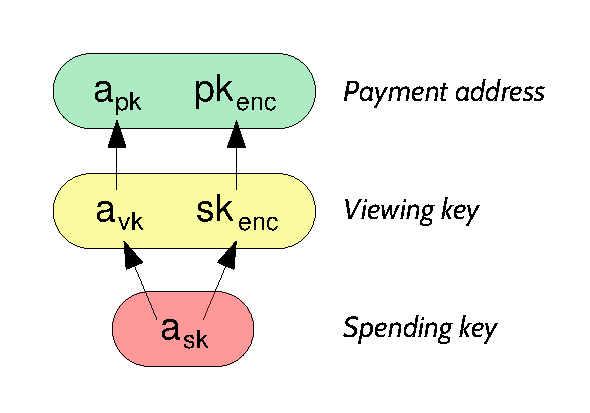
\includegraphics[scale=.7]{key_components}
\end{center}

The composition of \paymentAddresses\changed{, \viewingKeys,} and \spendingKeys
is a cryptographic protocol detail that should not normally be
exposed to users. However, user-visible operations should be provided
to obtain a \paymentAddress or \viewingKey from a \spendingKey.

Users can accept payment from multiple parties with a single \paymentAddress
$\PaymentAddress$ and the fact that these payments are destined to
the same payee is not revealed on the \blockchain, even to the
paying parties. \emph{However} if two parties collude to compare a
\paymentAddress they can trivially determine they are the same. In the
case that a payee wishes to prevent this they should create a distinct
\paymentAddress for each payer.

\subparagraph{Note:}
It is conventional in cryptography to refer to the key used to encrypt
a message in an asymmetric encryption scheme as the ``public key".
However, the public key used as the \transmissionKey component
of an address ($\TransmitPublic$) need not be publically distributed; it
has the same distribution as the \paymentAddress itself. As mentioned above,
limiting the distribution of the \paymentAddress is important for some use cases.
This also helps to reduce reliance of the overall protocol on the security
of the cryptosystem used for \note encryption (see \crossref{inband}), since
an adversary would have to know $\TransmitPublic$ in order to exploit a
hypothetical weakness in that cryptosystem.


\nsubsection{\Notes}

A \note (denoted $\NoteTuple{}$) is a tuple $\changed{(\AuthPublic, \Value,
\NoteAddressRand, \NoteCommitRand)}$. It represents that a value $\Value$ is
spendable by the recipient who holds the \spendingKey $\AuthPrivate$ corresponding
to $\AuthPublic$, as described in the previous section.

\begin{itemize}
    \item $\AuthPublic$ is a sequence of $\PRFOutputLength$ bits representing
        the \payingKey of the recipient.
    \item $\Value$ is an integer in the range $0 \leq \Value \leq \MAXMONEY$
        representing the value of the \note in \zatoshi
        ($1$ \ZEC = $10^8$ \zatoshi).
    \item $\NoteAddressRand$ is a sequence of $\PRFOutputLength$ bytes, which is
        used as input to $\PRFnf{\AuthPrivate}$ to obtain the \note's \nullifier.
    \item $\NoteCommitRand$ is a \commitmentTrapdoor.
\end{itemize}

$\NoteCommitRand$ is randomly generated by the sender. \changed{$\NoteAddressRand$
is generated from a random seed $\NoteAddressPreRand$ using
$\PRFrho{\NoteAddressPreRand}$.} Only a commitment to these values is disclosed
publicly, which allows the tokens $\NoteCommitRand$ and $\NoteAddressRand$ to blind
the value and recipient \emph{except} to those who possess these tokens.

\nsubsubsection{\NoteCommitments} \label{notecommitment}

The underlying $\Value$ and $\AuthPublic$ are blinded with $\NoteAddressRand$
and $\NoteCommitRand$. The resulting hash
$\cm = \NoteCommit(\NoteTuple{}) = \Commit{\NoteCommitRand}(\Value, \AuthPublic, \NoteAddressRand)$.

$\Commit{}$ is required to be a computationally binding and hiding commitment
scheme.

\nsubsubsection{\Nullifiers}

A \nullifier (denoted $\nf$) is derived from the $\NoteAddressRand$ component
of a \note as $\PRFnf{\AuthPrivate}(\NoteAddressRand)$. A \note is spent by proving
knowledge of $\NoteAddressRand$ and $\AuthPrivate$ in zero knowledge while
disclosing its \nullifier $\nf$, allowing $\nf$ to be used to prevent double-spending.

\nsubsubsection{\NotePlaintexts{} and \Memos}

Transmitted \notes are stored on the \blockchain in encrypted form, together with
a \noteCommitment $\cm$.

The \notePlaintexts in a \joinSplitDescription are encrypted to the
respective \transmissionKeys $\TransmitPublicNew{\allNew}$,
and the result forms part of a \notesCiphertext (see \crossref{inband}
for further details).

Each \notePlaintext (denoted $\NotePlaintext{}$) consists of
$(\Value, \NoteAddressRand, \NoteCommitRand\changed{, \Memo})$.

The first three of these fields are as defined earlier.

\changed{
$\Memo$ represents a \memo associated with this \note. The usage of the
\memo is by agreement between the sender and recipient of the \note.
}


\nsubsection{Transactions, Blocks, and the Block Chain}

At a given point in time, the \blockchainview of each \fullnode consists of a
sequence of one or more valid \blocks. Each \block consists of a sequence of one or
more \transactions. To each \transaction there is associated an initial \treestate,
which consists of a \noteCommitmentTree (\crossref{merkle}), \nullifierSet
(\crossref{nullifierset}), and data structures associated with \Bitcoin such as
the UTXO (Unspent Transaction Output) set.

Inputs to a \transaction insert value into a \term{value pool}, and outputs
remove value from this pool. As in \Bitcoin, the remaining value in the pool is
available to miners as a fee.

An \anchor is a Merkle tree root of a \noteCommitmentTree. It uniquely identifies
a \noteCommitmentTree state given the assumed security properties of the Merkle tree's
hash function. Since the \nullifierSet is always updated together with the
\noteCommitmentTree, this also identifies a particular state of the \nullifierSet.

In a given node's \blockchainview, \treestates are chained as follows:

\begin{itemize}
  \item The input \treestate of the first \block is the empty \treestate.
  \item The input \treestate of the first \transaction of a \block is the final
        \treestate of the immediately preceding \block.
  \item The input \treestate of each subsequent \transaction in a \block is the
        output \treestate of the immediately preceding \transaction.
  \item The final \treestate of a \block is the output \treestate of its last
        \transaction.
\end{itemize}

\daira{\joinSplitDescriptions also have input and output \treestates.}

We rely on Bitcoin-style consensus for \fullnodes to eventually converge on their
views of valid \blocks, and therefore of the sequence of \treestates in those
\blocks.


\nsubsection{\JoinSplitTransfers{} and Descriptions} \label{joinsplit}

A \joinSplitDescription is data included in a \transaction that describes a \joinSplitTransfer,
i.e.\ a confidential value transfer. This kind of value transfer is the primary
\Zcash-specific operation performed by \transactions; it uses, but should not be
confused with, the \joinSplitCircuit used for the \zkSNARK proof and verification.

A \joinSplitTransfer spends $\NOld$ \notes $\nOld{\allOld}$ and transparent input
$\vpubOld$, and creates $\NNew$ \notes $\nNew{\allNew}$ and transparent output
$\vpubNew$.

Each \transaction is associated with a \sequenceOfJoinSplitDescriptions.

The inputs and outputs of each \joinSplitTransfer{} \MUST balance exactly.
The \changed{total $\vpubNew$ value adds to, and the total} $\vpubOld$
value subtracts from the value pool of the containing \transaction.

\todo{Describe the interaction of transparent value flows with the \joinSplitDescription's
\changed{$\vpubOld$ and} $\vpubNew$.}

\changed{
The \anchor of each \joinSplitDescription in a \transaction must refer to either
some earlier \block's final \treestate, or to the output \treestate of any prior
\joinSplitDescription in the same \transaction.
}

These conditions act as constraints on the blocks that a \fullnode will
accept into its \blockchainview.


\nsubsection{\NoteCommitment{} Tree} \label{merkle}

\begin{center}
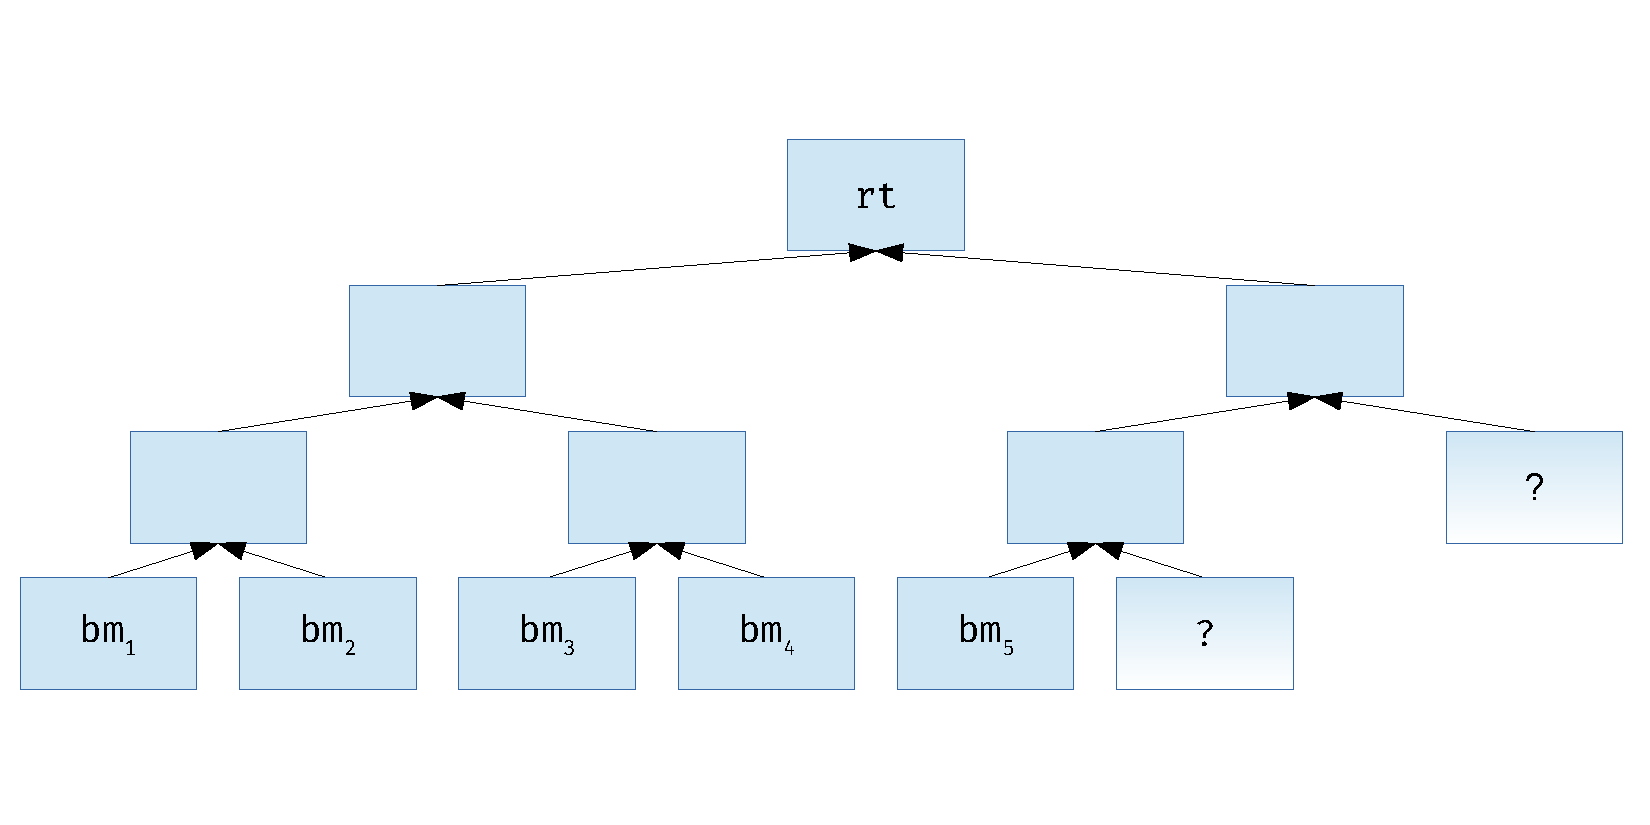
\includegraphics[scale=.4]{incremental_merkle}
\end{center}

The \noteCommitmentTree is an \incrementalMerkleTree of fixed depth used to
store \noteCommitments that \joinSplitTransfers produce. Just as the \term{unspent
transaction output set} (UTXO) used in \Bitcoin, it is used to express the existence
of value and the capability to spend it. However, unlike the UTXO, it is \emph{not}
the job of this tree to protect against double-spending, as it is append-only.

Blocks in the \blockchain are associated (by all nodes) with the \merkleRoot of this tree
after all of its constituent \joinSplitDescriptions' \noteCommitments have been
entered into the \noteCommitmentTree associated with the previous \block.
\daira{Make this more precise.}

Each \merkleNode in the \incrementalMerkleTree is associated with a \merkleHash of
size $\MerkleHashLength$ bytes.
The \merkleLayer numbered $h$, counting from \merkleLayer $0$ at the \merkleRoot, has
$2^h$ \merkleNodes with \merkleIndices $0$ to $2^h-1$ inclusive.
The \merkleHash associated with the \merkleNode at \merkleIndex $i$ in \merkleLayer $h$
is denoted $\MerkleNode{h}{i}$.


\nsubsection{\NullifierSet} \label{nullifierset}

Each \fullnode maintains a \nullifierSet alongside the \noteCommitmentTree and UTXO set.
As valid \transactions containing \joinSplitTransfers are processed, the \nullifiers
revealed in \joinSplitDescriptions are inserted into this \nullifierSet.

If a \joinSplitDescription reveals a \nullifier that already exists in
the \fullnode's \blockchainview, the containing transaction will be rejected, since
it would otherwise result in a double-spend.


\nsubsection{Coinbase Transactions}

The first \transaction in a block must be a \coinbaseTransaction, which should
collect and spend any block reward and transaction fees paid by \transactions
included in this block.

\nsubsubsection{Block Subsidy and Transaction Fees}

\todo{Describe money supply curve.}
\todo{Miner's reward = transaction fees + block subsidy - founder's reward}

\nsubsubsection{Coinbase outputs}

\todo{Coinbase maturity rule.}
\todo{Any tx with a coinbase input must have no transparent outputs (vout).}


\nsection{Abstract Protocol}

\nsubsection{Abstract Cryptographic Functions}

\nsubsubsection{Hash Functions} \label{abstracthashes}

$\MerkleCRH \typecolon \MerkleHash \times \MerkleHash \rightarrow \MerkleHash$
is a collision-resistant hash function used in \crossref{merkletree}.
It is instantiated in \crossref{merklecrh}.

\changed{
$\GeneralCRH{} \typecolon (\ell \typecolon 8\range{1}{64}) \times \GeneralCRHInput \rightarrow \bitseq{\ell}$
is another collision-resistant hash function. The first (subscripted) argument
indicates the output length in bits. It is used in \crossref{hsig} and
\crossref{equihash}, and instantiated in \crossref{generalcrh}.
}

\nsubsubsection{\PseudoRandomFunctions} \label{abstractprfs}

$\PRF{x}{}$ is a \pseudoRandomFunction keyed by $x$. \changed{Four} \emph{independent}
$\PRF{x}{}$ are needed in our protocol:

\begin{tabular}{@{\hskip 2em}l@{\;}l@{\;}l@{\;}l}
$\PRFaddr{} $&$\typecolon\; \bitseq{\AuthPrivateLength} $&$\times\; \range{0}{255} $&$\rightarrow \PRFOutput $\\
$\PRFnf{}   $&$\typecolon\; \bitseq{\AuthPrivateLength} $&$\times\; \PRFOutput $&$\rightarrow \PRFOutput $\\
$\PRFpk{}   $&$\typecolon\; \bitseq{\AuthPrivateLength} $&$\times\; \GeneralCRHOutput $&$\rightarrow \PRFOutput $\\
$\PRFrho{}  $&$\typecolon\; \bitseq{\NoteAddressPreRandLength} $&$\times\; \GeneralCRHOutput $&$\rightarrow \PRFOutput $
\end{tabular}

These are used in \crossref{circuit}; $\PRFaddr{}$ is also used to derive a \paymentAddress
from a \spendingKey in \crossref{keycomponents}.
They are instantiated in \crossref{concreteprfs}.

\securityrequirement{
In addition to being \pseudoRandomFunctions, it is required that $\PRFnf{x}$
\changed{, $\PRFaddr{x}$, and $\PRFrho{x}$} be collision-resistant across all $x$ ---
i.e.\ it should not be feasible to find $(x, y) \neq (x', y')$ such that
$\PRFnf{x}(y) = \PRFnf{x'}(y')$\changed{, and similarly for $\PRFaddr{}$ and $\PRFrho{}$}.
}

\nsubsubsection{\SymmetricEncryption} \label{abstractsym}

Let $\Sym$ be an \symmetricEncryptionScheme with keyspace $\Keyspace$, encrypting
plaintexts in $\Plaintext$ to produce ciphertexts in $\Ciphertext$.

$\SymEncrypt{} \typecolon \Keyspace \times \Plaintext \rightarrow \Ciphertext$
is the encryption algorithm.

$\SymDecrypt{} \typecolon \Keyspace \times \Ciphertext \rightarrow
\Plaintext \cup \setof{\bot}$ is the corresponding decryption algorithm, such that
for any $\Key \in \Keyspace$ and $\Ptext \in \Plaintext$,
$\SymDecrypt{\Key}(\SymEncrypt{\Key}(\Ptext)) = \Ptext$.
$\bot$ is used to represent the decryption of an invalid ciphertext.

\securityrequirement{
$\Sym$ must be one-time (INT-CTXT $\wedge$ IND-CPA)-secure. ``One-time'' here means
that an honest protocol participant will almost surely encrypt only one message with
a given key; however, the attacker may make many adaptive chosen ciphertext queries
for a given key. The security notions INT-CTXT and IND-CPA are as defined in
\cite{BN2007}.
}

%$\AuthEnc$ is an asymmetric authenticated encryption scheme. It consists of
%a randomized key pair generation algorithm $\AuthEncGen \typecolon () -> $,
%an encryption algorithm $\AuthEncEncrypt \typecolon \Nonce \times ...$,
%and a decryption algorithm $\AuthEncDecrypt$.

\nsubsubsection{\KeyAgreement} \label{abstractkeyagreement}

A \keyAgreementScheme is a cryptographic protocol in which two parties agree
a shared secret, each using their private key and the other party's public key.

A \keyAgreementScheme $\KA$ defines a type of public keys $\KAPublic$, a type
of private keys $\KAPrivate$, and a type of shared secrets $\KASharedSecret$.

Let $\KAFormatPrivate \typecolon \PRFOutput \rightarrow \KAPrivate$ be a function
that converts a bit string of length $\PRFOutputLength$ to a $\KA$ private key.

Let $\KADerivePublic \typecolon \KAPrivate \rightarrow \KAPublic$ be a function
that derives the $\KA$ public key corresponding to a given $\KA$ public key.

Let $\KAAgree \typecolon \KAPrivate \times \KAPublic \rightarrow \KASharedSecret$
be the agreement function.

\securityrequirement{
$\KAFormatPrivate$ must preserve sufficient entropy from its input to be used
as a secure $\KA$ private key. \todo{requirements on security of key agreement and KDF}
}


\nsubsubsection{\KeyDerivation} \label{abstractkdf}

A \keyDerivationFunction is defined for a particular \keyAgreementScheme and
\symmetricEncryptionScheme; it takes the shared secret produced by the key
agreement and additional arguments, and derives a key suitable for the encryption
scheme.

Let $\KDF \typecolon \setofNew \times \GeneralCRHOutput \times \KASharedSecret
\times \KAPublic \times \KAPublic \rightarrow \Keyspace$ be a
\keyDerivationFunction suitable for use with $\KA$, deriving keys
for $\SymEncrypt{}$.

\securityrequirement{
For any $T = (i \in \setofNew, \hSig \in \GeneralCRHOutput, \TransmitPublicNew{i} \in \KAPublic)$,
%let $\RandomVar{T}$ be 
\begin{itemize}
  \item[] $(\EphemeralPublic, \KDF(i, \hSig, \KAAgree(\EphemeralPrivate, \TransmitPublicNew{}),
                                   \EphemeralPublic, \TransmitPublicNew{}))$
          must be computationally indistinguishable between different
          $\TransmitPrivate \in \KAPrivate$,
  \item[] where $\EphemeralPublic = \KADerivePublic(\EphemeralPrivate)$ and
                $\TransmitPublicNew{} = \KADerivePublic(\TransmitPrivate)$.
\end{itemize}

This is necessary to ensure that the composition of $\KA$, $\KDF$ and $\Sym$ as
given in \crossref{inband} is a key-private asymmetric encryption scheme.
The property of key privacy is defined in \cite{BBDP2001}.
}

\nsubsubsection{Signatures} \label{abstractsig}

\todo{}

\nsubsection{Key Components} \label{keycomponents}

\changed{$\AuthPrivate$ is 252 bits.}
$\AuthPublic$, $\TransmitPrivate$, and $\TransmitPublic$, are each 256 bits.

Let $\KA$ be a \keyAgreementScheme, instantiated in \crossref{concretekeyagreement}.

\changed{
A new \spendingKey $\AuthPrivate$ is generated by sampling a bit string
uniformly at random from $\bitseq{\AuthPrivateLength}$.

$\AuthPublic$, $\TransmitPrivate$ and $\TransmitPublic$ are derived from
$\AuthPrivate$
as follows:}
{\hfuzz=50pt
\begin{equation*}
\begin{aligned}
\AuthPublic &:= \changed{\PRFaddr{\AuthPrivate}(0)} \\
\TransmitPrivate &:= \changed{\KAFormatPrivate(\PRFaddr{\AuthPrivate}(1))} \\
\TransmitPublic &:= \changed{\KADerivePublic(\TransmitPrivate)}
\end{aligned}
\end{equation*}
}

\changed{
where
\begin{itemize}
  \item $\CurveMultiply(\bytes{n}, \bytes{q})$ performs point
multiplication of the Curve25519 public key represented by the byte
sequence $\bytes{q}$ by the Curve25519 secret key represented by the
byte sequence $\bytes{n}$, as defined in \cite[section 2]{Bern2006};
  \item $\CurveBase$ is the public byte sequence representing the Curve25519
base point;
  \item $\Clamp(\bytes{x})$ takes a 32-byte sequence $\bytes{x}$ as input
and returns a byte sequence representing a Curve25519 private key, with
bits ``clamped'' as described in \cite[section 3]{Bern2006}:
``clear bits $0, 1, 2$ of the first byte, clear bit $7$ of the last byte,
and set bit $6$ of the last byte.'' Here the bits of a byte are numbered
such that bit $b$ has numeric weight $2^b$.
\end{itemize}
}

\nsubsection{Note Components}

\begin{itemize}
    \item $\AuthPublic$ is a 32-byte \payingKey of the recipient.
    \item $\Value$ is a 64-bit unsigned integer representing the value of the
        \note in \zatoshi ($1$ \ZEC = $10^8$ \zatoshi).
    \item $\NoteAddressRand$ is a 32-byte $\PRFnf{\AuthPrivate}$ preimage.
    \item $\NoteCommitRand$ is a 32-byte \commitmentTrapdoor.
\end{itemize}

\nsubsection{\JoinSplitTransfers{} and Descriptions} \label{joinsplitdesc}

A \joinSplitDescription is data included in a \transaction that describes a
\joinSplitTransfer, as described in \crossref{joinsplit}.

\changed{
\Zcash \transactions have the following additional fields:

\begin{center}
\hbadness=4000
\begin{tabularx}{0.92\textwidth}{|c|l|p{10.7em}|X|}
\hline
Bytes & \heading{Name} & \heading{Data Type} & \heading{Description} \\
\hhline{|=|=|=|=|}

\Varies & $\nJoinSplit$ & \type{compactSize uint} & The number of \joinSplitDescriptions
in $\vJoinSplit$. \\ \hline

1802 $\times\, \nJoinSplit$ & $\vJoinSplit$ &
\type{JoinSplitDescription} \type{[$\nJoinSplit$]} &
The \sequenceOfJoinSplitDescriptions in this \transaction. \\ \hline

32 $\dagger$ & $\joinSplitPubKey$ & \type{char[32]} & An encoding of a $\JoinSplitSigAlg$
public verification key. \\ \hline

64 $\dagger$ & $\joinSplitSig$ & \type{char[64]} & A signature on a prefix of the \transaction encoding,
to be verified using $\joinSplitPubKey$. \\ \hline
\end{tabularx}
\end{center}

$\dagger$ The $\joinSplitPubKey$ and $\joinSplitSig$ fields are present if and only if
$\nJoinSplit > 0$.

The encoding of $\joinSplitPubKey$ and the data to be signed are specified in
\crossref{nonmalleability}.
}

Each \type{JoinSplitDescription} consists of:

\begin{center}
\hbadness=2000
\begin{tabularx}{0.92\textwidth}{|c|l|l|X|}
\hline
Bytes & \heading{Name} & \heading{Data Type} & \heading{Description} \\
\hhline{|=|=|=|=|}

\setchanged 8 &\setchanged $\vpubOldField$ &\setchanged \type{int64\_t} &\mbox{}\setchanged
A value $\vpubOld$ that the \joinSplitTransfer removes from the value pool. \\ \hline

8 & $\vpubNewField$ & \type{int64\_t} & A value $\vpubNew$ that the \joinSplitTransfer inserts
into the value pool. \\ \hline

32 & $\anchorField$ & \type{char[32]} & A merkle root $\rt$ of the \noteCommitmentTree at
some block height in the past, or the merkle root produced by a previous \joinSplitTransfer in
this \transaction. \sean{We need to be more specific here.} \\ \hline

64 & $\nullifiersField$ & \type{char[32][$\NOld$]} & A sequence of \nullifiers of the input
\notes $\nfOld{\allOld}$. \\ \hline

64 & $\commitments$ & \type{char[32][$\NNew$]}. & A sequence of \noteCommitments for the
output \notes $\cmNew{\allNew}$. \\ \hline

\setchanged 32 &\setchanged $\ephemeralKey$ &\setchanged \type{char[32]} &\mbox{}\setchanged
A Curve25519 public key $\EphemeralPublic$. \\ \hline

\setchanged 32 &\setchanged $\randomSeed$ &\setchanged \type{char[32]} &\mbox{}\setchanged
A 256-bit seed that must be chosen independently at random for each \joinSplitDescription. \\ \hline

64 & $\vmacs$ & \type{char[32][$\NOld$]} & A sequence of message authentication tags
$\h{\allOld}$ that bind $\hSig$ to each $\AuthPrivate$ of the
$\joinSplitDescription$. \\ \hline

296 & $\zkproof$ & \type{char[296]} & An encoding of the zero-knowledge proof $\JoinSplitProof$
(\crossref{proofencoding}). \\ \hline

1202 & $\encCiphertexts$ & \type{char[601][$\NNew$]} & A sequence of ciphertext
components for the encrypted output \notes, $\TransmitCiphertext{\allNew}$. \\ \hline

\end{tabularx}
\end{center}

The $\ephemeralKey$ and $\encCiphertexts$ fields together form the \notesCiphertext.

\consensusrule{
$0 \leq \vpubOld \leq \MAXMONEY$, and $0 \leq \vpubNew \leq \MAXMONEY$.
}

\consensusrule{
Either $\vpubOld$ or $\vpubNew$ \MUST be zero.
}

\todo{Describe case where there are fewer than $\NOld$ real input \notes.}

\nsubsubsection{Computation of \hSigText} \label{hsig}

\newsavebox{\hsigbox}
\begin{lrbox}{\hsigbox}
\setchanged
\begin{bytefield}[bitwidth=0.04em]{1024}
    \bitbox{256}{$256$-bit $\RandomSeed$}
    \bitbox{256}{\hfill $256$-bit $\nfOld{\mathrm{1}}$\hfill...\;} &
    \bitbox{256}{$256$-bit $\nfOld{\NOld}$} &
    \bitbox{256}{$256$-bit $\joinSplitPubKey$}
\end{bytefield}
\end{lrbox}

\changed{
Given a \joinSplitDescription containing the fields $\randomSeed$ and
$\nullifiersField = \nfOld{\allOld}$, and embedded in a transaction
containing the field $\joinSplitPubKey$, we compute $\hSig$ for that
\joinSplitDescription as follows:
\begin{equation*}
\begin{aligned}
\hSigInput &:= \Justthebox{\hsigbox} \\
\hSig &:= \GeneralCRH{256}(\ascii{ZcashComputehSig},\; \hSigInput)
\end{aligned}
\end{equation*}
}

\nsubsubsection{Merkle root validity} \label{merkletree}

\daira{This paragraph is confusing and only describes one aspect of validity.}
A \joinSplitDescription is valid if $\rt$ is a \noteCommitmentTree root found in
either the blockchain or a merkle root produced by inserting the \noteCommitments
of a previous \joinSplitDescription in the \transaction to the \noteCommitmentTree
identified by that previous \joinSplitDescription's $\anchor$.

The depth of the \noteCommitmentTree is $\MerkleDepth$.

Each \merkleNode in the \incrementalMerkleTree is associated with a \merkleHash,
which is a byte sequence. The \merkleLayer numbered $h$, counting from
\merkleLayer $0$ at the \merkleRoot, has $2^h$ \merkleNodes with \merkleIndices
$0$ to $2^h-1$ inclusive.

Let $\MerkleNode{h}{i}$ be the \merkleHash associated with the \merkleNode at
\merkleIndex $i$ in \merkleLayer $h$.

The \merkleNodes at \merkleLayer $\MerkleDepth$ are called \merkleLeafNodes.
When a \noteCommitment is added to the tree, it occupies the \merkleLeafNode
\merkleHash $\MerkleNode{\MerkleDepth}{i}$ for the next available $i$. As-yet unused
\merkleLeafNodes are associated with a distinguished \merkleHash $\Uncommitted$.
It is assumed to be infeasible to find a preimage \note $\NoteTuple{}$ such that
$\NoteCommit(\NoteTuple{}) = \Uncommitted$.

The \merkleNodes at \merkleLayers $0$ to $\MerkleDepth-1$ inclusive are called
\merkleInternalNodes, and are associated with $\MerkleCRH$ outputs.
\MerkleInternalNodes are computed from their children in the next \merkleLayer
as follows: for $0 \leq h < \MerkleDepth$ and $0 \leq i < 2^h$,

\hskip 2em $\MerkleNode{h}{i} := \MerkleCRH(\MerkleNode{h+1}{2i}, \MerkleNode{h+1}{2i+1})$.

A \merklePath from \merkleLeafNode $\MerkleNode{\MerkleDepth}{i}$ in the
\incrementalMerkleTree is the sequence

\hskip 2em $[\hairspace\MerkleNode{h}{\MerkleSibling(h, i)} \text{ for }
h \text{ from } \MerkleDepth \text{ down to } 1\hairspace]$,

where

\hskip 2em $\MerkleSibling(h, i) = \floor{\frac{i}{2^{\MerkleDepth-h}}} \xor 1$

Given such a \merklePath, it is possible to verify that \merkleLeafNode
$\MerkleNode{\MerkleDepth}{i}$ is in a tree with a given \merkleRoot $\rt = \MerkleNode{0}{0}$.

\nsubsubsection{Non-malleability} \label{nonmalleability}

\changed{
\Bitcoin defines several \sighashTypes that cover various parts of a transaction.
In \Zcash, all of these \sighashTypes are extended to cover the \Zcash-specific
fields $\nJoinSplit$, $\vJoinSplit$, and (if present) $\joinSplitPubKey$.
They \emph{do not} cover the field $\joinSplitSig$.

\consensusrule{
If $\nJoinSplit > 0$, the \transaction{} \MUSTNOT use \sighashTypes other than
$\SIGHASHALL$.
}

Let $\dataToBeSigned$ be the hash of the \transaction using the $\SIGHASHALL$
\sighashType. This \emph{excludes} all of the $\scriptSig$ fields in
the non-\Zcash-specific parts of the \transaction.

In order to ensure that a \joinSplitDescription is cryptographically bound to the
transparent inputs and outputs corresponding to $\vpubNew$ and $\vpubOld$, and
to the other \joinSplitDescriptions in the same \transaction, an ephemeral $\JoinSplitSigAlg$
key pair is generated for each \transaction, and the $\dataToBeSigned$ is
signed with the private signing key of this key pair. The corresponding public
verification key is included in the \transaction encoding as $\joinSplitPubKey$.

$\JoinSplitSigAlg$ is instantiated as $\JoinSplitSigSpecific$ \cite{BDL+2012},
with the additional requirement that $\EdDSAs$ (the integer represented
by $\EdDSAS$) must be less than the prime
$\ell = 2^{252} + 27742317777372353535851937790883648493$,
otherwise the signature is considered invalid.
$\JoinSplitSigSpecific$ is defined as using $\JoinSplitSigHashName$ internally.

If $\nJoinSplit$ is zero, the $\joinSplitPubKey$ and $\joinSplitSig$ fields are
omitted. Otherwise, a \transaction has a correct \joinSplitSignature if
$\joinSplitSig$ can be verified as an encoding of a signature on $\dataToBeSigned$
as specified above, using the $\JoinSplitSigSpecific$ public key encoded as
$\joinSplitPubKey$.
}

\newsavebox{\sigbox}
\begin{lrbox}{\sigbox}
\setchanged
\begin{bytefield}[bitwidth=0.075em]{512}
    \bitbox{256}{$256$-bit $\EdDSAR$}
    \bitbox{256}{$256$-bit $\EdDSAS$}
\end{bytefield}
\end{lrbox}

\changed{
The encoding of a signature is:
}
\begin{itemize}
  \item[] $\Justthebox{\sigbox}$
\end{itemize}

\changed{
where $\EdDSAR$ and $\EdDSAS$ are as defined in \cite{BDL+2012}.

The encoding of a public key is as defined in \cite{BDL+2012}.
}

The condition enforced by the \joinSplitCircuit specified in \crossref{nonmalleablepour}
ensures that a holder of all of $\AuthPrivateOld{\allOld}$ for each
\joinSplitDescription has authorized the use of the private signing key corresponding
to $\joinSplitPubKey$ to sign this \transaction.


\nsubsubsection{Balance}

A \joinSplitTransfer can be seen, from the perspective of the \transaction, as
an input \changed{and an output simultaneously}.
\changed{$\vpubOld$ takes value from the value pool and}
$\vpubNew$ adds value to the value pool. As a result, \changed{$\vpubOld$ is
treated like an \emph{output} value, whereas} $\vpubNew$ is treated like an
\emph{input} value.

\changed{
\subparagraph{Note:}
Unlike original \Zerocash \cite{BCG+2014}, \Zcash does not have
a distinction between Mint and Pour operations. The addition of $\vpubOld$ to a
\joinSplitDescription subsumes the functionality of both Mint and Pour. Also,
\joinSplitDescriptions are indistinguishable regardless of the number of real input
\notes.

As stated in \crossref{joinsplitdesc}, either $\vpubOld$ or $\vpubNew$ \MUST be zero.
No generality is lost because, if a \transaction in which both $\vpubOld$ and
$\vpubNew$ were nonzero were allowed, it could be replaced by an equivalent one
in which $\minimum(\vpubOld, \vpubNew)$ is subtracted from both of these values.
This restriction helps to avoid unnecessary distinctions between \transactions
according to client implementation.
}

\nsubsubsection{\NoteCommitments{} and \Nullifiers}

A \transaction that contains one or more \joinSplitDescriptions, when entered into the
blockchain, appends to the \noteCommitmentTree with all constituent
\noteCommitments. All of the constituent \nullifiers are also entered into the
\nullifierSet of the \blockchainview \emph{and} \mempool. A \transaction is not
valid if it attempts to add a \nullifier to the \nullifierSet that already
exists in the set.

\nsubsubsection{\JoinSplitCircuit{}} \label{circuit}

A valid instance of $\JoinSplitProof$ assures that given a \term{primary input}:

\begin{itemize}
  \item[] $(\rt, \nfOld{\allOld}, \cmNew{\allNew}, \changed{\vpubOld,\;}
\vpubNew, \hSig, \h{\allOld})$,
\end{itemize}

there exists a witness of \term{auxiliary input}:

\begin{itemize}
  \item[] $(\treepath{\allOld}, \nOld{\allOld}, \AuthPrivateOld{\allOld},
\nNew{\allNew}\changed{, \NoteAddressPreRand})$
\end{itemize}

where:

\begin{itemize}
  \item[] for each $i \in \setofOld$: $\nOld{i} = (\AuthPublicOld{i},
\vOld{i}, \NoteAddressRandOld{i}, \NoteCommitRandOld{i})$;
  \item[] for each $i \in \setofNew$: $\nNew{i} = (\AuthPublicNew{i},
\vNew{i}, \NoteAddressRandNew{i}, \NoteCommitRandNew{i})$
\end{itemize}

such that the following conditions hold:

\subparagraph{Merkle path validity} \label{merklepathvalidity}

for each $i \in \setofOld$ \changed{$\mid$ $\vOld{i} \neq 0$}:
$\treepath{i}$ must be a valid \merklePath of depth $\MerkleDepth$, as defined in
\crossref{merkle}, from $\NoteCommit(\nOld{i})$ to \noteCommitmentTree root $\rt$.

\textbf{Note:} Merkle path validity covers both conditions 1. (a) and 1. (d) of the NP statement
given in \cite[section 4.2]{BCG+2014}.

\subparagraph{Balance}

$\changed{\vpubOld\; +} \vsum{i=1}{\NOld} \vOld{i} = \vpubNew + \vsum{i=1}{\NNew} \vNew{i}$.

\subparagraph{\Nullifier{} integrity}

for each $i \in \setofNew$:
$\nfOld{i} = \PRFnf{\AuthPrivateOld{i}}(\NoteAddressRandOld{i})$.

\subparagraph{Spend authority} \label{spendauthority}

for each $i \in \setofOld$:
$\AuthPublicOld{i} = \changed{\PRFaddr{\AuthPrivateOld{i}}(0)}$.

\subparagraph{Non-malleability} \label{nonmalleablepour}

for each $i \in \setofOld$:
$\h{i} = \PRFpk{\AuthPrivateOld{i}}(i, \hSig)$.

\changed{
\subparagraph{Uniqueness of $\NoteAddressRandNew{i}$} \label{uniquerho}

for each $i \in \setofNew$:
$\NoteAddressRandNew{i} = \PRFrho{\NoteAddressPreRand}(i, \hSig)$.
}

\subparagraph{Commitment integrity}

for each $i \in \setofNew$: $\cmNew{i}$ = $\NoteCommit(\nNew{i})$.

\vspace{2.5ex}
For details of the form and encoding of proofs, see \crossref{proofs}.


\nsubsection{In-band secret distribution} \label{inband}

In order to transmit the secret $\Value$, $\NoteAddressRand$, and $\NoteCommitRand$
(necessary for the recipient to later spend) \changed{and also a \memo} to the
recipient \emph{without} requiring an out-of-band communication channel, the
\transmissionKey $\TransmitPublic$ is used to encrypt these
secrets. The recipient's possession of the associated \keyTuple
$(\AuthPrivate, \TransmitPrivate, \PaymentAddress)$ is used to reconstruct
the original \note \changed{ and \memo}.

All of the resulting ciphertexts are combined to form a \notesCiphertext.

\nsubsubsection{Encryption}

\changed{
Let $\SymEncrypt{\Key}(\Ptext)$ be authenticated encryption using
$\SymSpecific$ \cite{RFC-7539} encryption of plaintext $\Ptext \in \Plaintext$,
with empty ``associated data", all-zero nonce $\zeros{96}$, and 256-bit key
$\Key \in \Keyspace$.

Similarly, let $\SymDecrypt{\Key}(\Ctext)$ be $\SymSpecific$
decryption of ciphertext $\Ctext \in \Ciphertext$, with empty
``associated data", all-zero nonce $\zeros{96}$, and 256-bit key
$\Key \in \Keyspace$. The result is either the plaintext byte sequence,
or $\bot$ indicating failure to decrypt.
}

Let $\TransmitPublicNew{\allNew}$ be the \changed{Curve25519} public keys
for the intended recipient addresses of each new \note, and let
$\NotePlaintext{\allNew}$ be the \notePlaintexts as defined in \crossref{notept}.
Let $\hSig$ be the value computed in \crossref{hsig}. Let $\KDF$ be the
\keyDerivationFunction instantiated in \crossref{concretekdf}.

Then to encrypt:
\begin{itemize}
\changed{
  \item Generate a new Curve25519 (public, private) key pair
$(\EphemeralPublic, \EphemeralPrivate)$.
  \item For $i \in \setofNew$,
    \begin{itemize}
      \item Let $\TransmitPlaintext{i}$ be the raw encoding of $\NotePlaintext{i}$.
      \item Let $\DHSecret{i} := \CurveMultiply(\EphemeralPrivate,
\TransmitPublicNew{i})$.
      \item Let $\TransmitKey{i} := \KDF(i, \hSig, \DHSecret{i}, \EphemeralPublic,
\TransmitPublicNew{i})$.
      \item Let $\TransmitCiphertext{i} :=
\SymEncrypt{\TransmitKey{i}}(\TransmitPlaintext{i})$.
    \end{itemize}
}
\end{itemize}

The resulting \notesCiphertext is $\changed{(\EphemeralPublic,
\TransmitCiphertext{\allNew})}$.

\nsubsubsection{Decryption by a Recipient}

Let $\PaymentAddress = (\AuthPublic, \TransmitPublic)$ be the recipient's
\paymentAddress, and let $\TransmitPrivate$ be the recipient's \viewingKey.
Let $\hSig$ be the value computed in \crossref{hsig}.
Let $\cmNew{\allNew}$ be the \noteCommitments of each output coin.
Then for each $i \in \setofNew$, the recipient will attempt to decrypt that ciphertext
component as follows:

\changed{
\begin{itemize}
  \item Let $\DHSecret{i} := \CurveMultiply(\TransmitPrivate, \EphemeralPublic)$.
  \item Let $\TransmitKey{i} := \KDF(i, \hSig, \DHSecret{i}, \EphemeralPublic,
\TransmitPublicNew{i})$.
  \item Return $\DecryptNote(\TransmitKey{i}, \TransmitCiphertext{i}, \cmNew{i},
\AuthPublic).$
\end{itemize}

$\DecryptNote(\TransmitKey{i}, \TransmitCiphertext{i}, \cmNew{i}, \AuthPublic)$
is defined as follows:

\begin{itemize}
  \item Let $\TransmitPlaintext{i} :=
\SymDecrypt{\TransmitKey{i}}(\TransmitCiphertext{i})$.
  \item If $\TransmitPlaintext{i} = \bot$, return $\bot$.
  \item Extract $\NotePlaintext{i} = (\ValueNew{i},
\NoteAddressRandNew{i}, \NoteCommitRandNew{i}, \Memo_i)$ from $\TransmitPlaintext{i}$.
  \item If $\NoteCommit((\AuthPublic, \ValueNew{i}, \NoteAddressRandNew{i},
\NoteCommitRandNew{i})) \neq \cmNew{i}$, return $\bot$, else return $\NotePlaintext{i}$.
\end{itemize}
}

\textbf{Note:} This corresponds to step 3 (b) i. and ii. (first bullet point) of the
$\Receive$ algorithm shown in \cite[Figure 2]{BCG+2014}.

To test whether a \note is unspent in a particular \blockchainview also requires
the \spendingKey $\AuthPrivate$; the coin is unspent if and only if
$\nf = \PRFnf{\AuthPrivate}(\NoteAddressRand)$ is not in the \nullifierSet
for that \blockchainview.

\subparagraph{Notes:}
\begin{itemize}
  \item A \note can change from being unspent to spent on a given \blockchainview,
as \transactions are added to that view. Also, blockchain reorganisations can cause
the \transaction in which a \note was output to no longer be on the consensus
blockchain.
  \item The nonce parameter to $\SymSpecific$ is not used.
  \item The ``IETF" definition of $\SymSpecific$ from \cite{RFC-7539} is
used; this uses a 32-bit block count and a 96-bit nonce, rather than a 64-bit
block count and 64-bit nonce as in the original definition of $\SymCipher$.
\end{itemize}

See \crossref{inbandrationale} for further discussion of the security and
engineering rationale behind this encryption scheme.


\nsection{Concrete Protocol}

\nsubsection{Integers, Bit Sequences, and Endianness} \label{boxnotation}

All integers in \emph{\Zcash-specific} encodings are unsigned, have a fixed
bit length, and are encoded in little-endian byte order \emph{unless otherwise
specified}.

In bit layout diagrams, each box of the diagram represents a sequence of bits.
Diagrams are read from left-to-right, with lines read from top-to-bottom;
the breaking of boxes across lines has no significance.
The bit length is given explicitly in each box, except for the case of a single
bit, or for the notation $\zeros{n}$ which represents the sequence of $n$ zero bits.

The entire diagram represents the sequence of \emph{bytes} formed by first
concatenating these bit sequences, and then treating each subsequence of 8 bits
as a byte with the bits ordered from \emph{most significant} to
\emph{least significant}. Thus the \emph{most significant} bit in each byte
is toward the left of a diagram. Where bit fields are used, the text will
clarify their position in each case.

\begin{comment}
\todo{Update example for big-bit-endian order.}

\newsavebox{\exampleabox}
\begin{lrbox}{\exampleabox}
\setchanged
\begin{bytefield}[bitwidth=1.3em]{32}
        \bitbox{1}{0} &
        \bitbox{1}{1} &
        \bitbox{1}{0} &
        \bitbox{1}{0} &
        \bitbox{16}{16 bit $\hexint{ABCD}$} &
        \bitbox{12}{12 bit $\hexint{123}$} &
\end{bytefield}
\end{lrbox}

\newsavebox{\examplebbox}
\begin{lrbox}{\examplebbox}
\setchanged
\begin{bytefield}[bitwidth=1.3em]{32}
        \bitbox{4}{4 bit $\hexint{2}$} &
        \bitbox{4}{4 bit $\hexint{D}$} &
        \bitbox{4}{4 bit $\hexint{C}$} &
        \bitbox{4}{4 bit $\hexint{B}$} &
        \bitbox{4}{4 bit $\hexint{A}$} &
        \bitbox{4}{4 bit $\hexint{3}$} &
        \bitbox{4}{4 bit $\hexint{2}$} &
        \bitbox{4}{4 bit $\hexint{1}$} &
\end{bytefield}
\end{lrbox}

\newsavebox{\examplecbox}
\begin{lrbox}{\examplecbox}
\setchanged
\begin{bytefield}[bitwidth=1.3em]{32}
        \bitbox{8}{8 bit $\hexint{D2}$} &
        \bitbox{8}{8 bit $\hexint{BC}$} &
        \bitbox{8}{8 bit $\hexint{3A}$} &
        \bitbox{8}{8 bit $\hexint{12}$} &
\end{bytefield}
\end{lrbox}

For example, the following diagrams are all equivalent:
\begin{itemize}
  \item[] $\Justthebox{\exampleabox}$
  \item[] $\Justthebox{\examplebbox}$
  \item[] $\Justthebox{\examplecbox}$
\end{itemize}

and represent the byte sequence $[\hexint{D2}, \hexint{BC}, \hexint{3A}, \hexint{12}]$.
\end{comment}

\nsubsection{Constants} \label{constants}

Define:

\begin{itemize}
  \item[] $\MerkleDepth = 32$
  \item[] $\NOld = 2$
  \item[] $\NNew = 2$
  \item[] $\MerkleHashLength = 256$
  \item[] $\GeneralCRHLength = 256$
  \item[] $\PRFOutputLength = 256$
  \item[] $\NoteCommitRandLength = 256$
  \item[] $\RandomSeedLength = 256$
  \item[] $\AuthPrivateLength = 252$
  \item[] $\NoteAddressPreRandLength = 252$
  \item[] $\Uncommitted = \zeros{\MerkleHashLength}$
  \item[] $\MAXMONEY = 2.1 \times 10^{15}$.
\end{itemize}


\nsubsection{Concrete Cryptographic Functions}

\nsubsubsection{Merkle Tree Hash Function} \label{merklecrh}

$\MerkleCRH$ is used to hash \incrementalMerkleTree \merkleHashes.
It is instantiated by the $\SHAName$ function, which takes a 512-bit block
and produces a 256-bit hash. \cite{NIST2015}

\newsavebox{\merklebox}
\begin{lrbox}{\merklebox}
\begin{bytefield}[bitwidth=0.04em]{512}
    \bitbox{256}{$256$-bit $\mathsf{left}$} &
    \bitbox{256}{$256$-bit $\mathsf{right}$}
\end{bytefield}
\end{lrbox}

\hskip 2em $\MerkleCRH(\mathsf{left}, \mathsf{right}) := \CRHbox{\merklebox}$.

\subparagraph{Note:}
$\SHA$ is not the same as the $\FullHashName$ function, which hashes arbitrary-length
sequences.

\securityrequirement{
$\SHA$ must be collision-resistant, and it must be infeasible to find a preimage $x$
such that $\SHA(x) = \zeros{256}$.
}

\nsubsubsection{General Hash Function} \label{generalcrh}

\changed{
$\GeneralCRH{\ell}$ is a collision-resistant hash function, producing outputs of
length $\ell \typecolon 8\range{1}{64}$ bits. It is used in \crossref{hsig} and
\crossref{equihash}.

$\GeneralCRH{\ell}(p, x)$ is instantiated by unkeyed $\Blake{\ell}$, that is,
$\BlakeGeneric$ as defined in \cite{ANWW2013}, with an output digest length of
$\ell/8$ bytes, 16-byte personalization string $p$, and input $x$.

\subparagraph{Note:}
$\Blake{\ell}$ is not the same as $\Blake{512}$ truncated to $\ell$ bits.

\securityrequirement{
$\Blake{\ell}(p, x)$ must be collision-resistant, for any $\ell$ and $p$
used in the protocol.
}
}

\nsubsubsection{\PseudoRandomFunctions} \label{concreteprfs}

The \changed{four} independent PRFs described in \crossref{abstractprfs} are
all instantiated using the $\SHAName$ function:

\newcommand{\iminusone}{\hspace{0.3pt}\scriptsize{$i$\hspace{0.6pt}-1}}

\newsavebox{\addrbox}
\begin{lrbox}{\addrbox}
\setchanged
\begin{bytefield}[bitwidth=0.06em]{512}
    \bitbox{18}{$1$} &
    \bitbox{18}{$1$} &
    \bitbox{18}{$0$} &
    \bitbox{18}{$0$} &
    \bitbox{224}{$252$-bit $x$} &
    \bitbox{56}{$8$-bit $t$} &
    \bitbox{200}{$\zeros{248}$}
\end{bytefield}
\end{lrbox}

\newsavebox{\nfbox}
\begin{lrbox}{\nfbox}
\setchanged
\begin{bytefield}[bitwidth=0.06em]{512}
    \bitbox{18}{$1$} &
    \bitbox{18}{$1$} &
    \bitbox{18}{$1$} &
    \bitbox{18}{$0$} &
    \bitbox{224}{$252$-bit $\AuthPrivate$} &
    \bitbox{256}{$256$-bit $\NoteAddressRand$}
\end{bytefield}
\end{lrbox}

\newsavebox{\pkbox}
\begin{lrbox}{\pkbox}
\setchanged
\begin{bytefield}[bitwidth=0.06em]{512}
    \bitbox{18}{$0$} &
    \bitbox{18}{\iminusone} &
    \bitbox{18}{$0$} &
    \bitbox{18}{$0$} &
    \bitbox{224}{$252$-bit $\AuthPrivate$} &
    \bitbox{256}{$256$-bit $\hSig$}
\end{bytefield}
\end{lrbox}

\newsavebox{\rhobox}
\begin{lrbox}{\rhobox}
\setchanged
\begin{bytefield}[bitwidth=0.06em]{512}
    \bitbox{18}{$0$} &
    \bitbox{18}{\iminusone} &
    \bitbox{18}{$1$} &
    \bitbox{18}{$0$} &
    \bitbox{224}{$252$-bit $\NoteAddressPreRand$} &
    \bitbox{256}{$256$-bit $\hSig$}
\end{bytefield}
\end{lrbox}

\begin{equation*}
\begin{aligned}
\setchanged \PRFaddr{x}(t) &\setchanged := \CRHbox{\addrbox} \\
\PRFnf{\AuthPrivate}(\NoteAddressRand) &:= \CRHbox{\nfbox} \\
\PRFpk{\AuthPrivate}(i, \hSig) &:= \CRHbox{\pkbox} \\
\setchanged \PRFrho{\NoteAddressPreRand}(i, \hSig) &\setchanged := \CRHbox{\rhobox}
\end{aligned}
\end{equation*}

\begin{securityrequirements}
  \item The $\SHAName$ function must be collision-resistant.
  \item The $\SHAName$ function must be a PRF when keyed by the bits
        corresponding to $x$, $\AuthPrivate$ or $\NoteAddressPreRand$
        in the above diagrams, with input in the remaining bits.
\end{securityrequirements}

\changed{
\subparagraph{Note:}
The first four bits --i.e.\ the most significant four bits of the first byte--
are used to distinguish different uses of $\SHA$, ensuring that the functions
are independent. In addition to the inputs shown here, the bits $\mathtt{1011}$
in this position are used to distinguish uses of the full $\FullHashName$ hash
function --- see \crossref{concretecomm}.
(The specific bit patterns chosen here are motivated by the possibility of future
extensions that either increase $\NOld$ and/or $\NNew$ to 3, or that add an
additional bit to $\AuthPrivate$ to encode a new key type, or that require an
additional PRF.)
}

\nsubsubsection{\SymmetricEncryption} \label{concretesym}

Let $\Sym$ be an \symmetricEncryptionScheme with keyspace $\Keyspace$, encrypting
plaintexts in $\Plaintext$ to produce ciphertexts in $\Ciphertext$.

$\SymEncrypt{} \typecolon \Keyspace \times \Plaintext \rightarrow \Ciphertext$
is the encryption algorithm.

$\SymDecrypt{} \typecolon \Keyspace \times \Ciphertext \rightarrow
\Plaintext \cup \setof{\bot}$ is the corresponding decryption algorithm, such that
for any $\Key \in \Keyspace$ and $\Ptext \in \Plaintext$,
$\SymDecrypt{\Key}(\SymEncrypt{\Key}(\Ptext)) = \Ptext$.
$\bot$ is used to represent the decryption of an invalid ciphertext.

\securityrequirement{
$\Sym$ must be one-time (INT-CTXT $\wedge$ IND-CPA)-secure. ``One-time'' here means
that an honest protocol participant will almost surely encrypt only one message with
a given key; however, the attacker may make many adaptive chosen ciphertext queries
for a given key. The security notions INT-CTXT and IND-CPA are as defined in
\cite{BN2007}.
}

\nsubsubsection{\KeyAgreement} \label{concretekeyagreement}

A \keyAgreementScheme is a cryptographic protocol in which two parties agree
a shared secret, each using their private key and the other party's public key.

A \keyAgreementScheme $\KA$ defines a type of public keys $\KAPublic$, a type
of private keys $\KAPrivate$, and a type of shared secrets $\KASharedSecret$.

Let $\KAFormatPrivate \typecolon \PRFOutput \rightarrow \KAPrivate$ be a function
that converts a bit string of length $\PRFOutputLength$ to a $\KA$ private key.

Let $\KADerivePublic \typecolon \KAPrivate \rightarrow \KAPublic$ be a function
that derives the $\KA$ public key corresponding to a given $\KA$ public key.

Let $\KAAgree \typecolon \KAPrivate \times \KAPublic \rightarrow \KASharedSecret$
be the agreement function.

\securityrequirement{
$\KAFormatPrivate$ must preserve sufficient entropy from its input to be used
as a secure $\KA$ private key. \todo{requirements on security of key agreement and KDF}
}

\changed{
where
\begin{itemize}
  \item $\CurveMultiply(\bytes{n}, \bytes{q})$ performs point
multiplication of the Curve25519 public key represented by the byte
sequence $\bytes{q}$ by the Curve25519 secret key represented by the
byte sequence $\bytes{n}$, as defined in \cite[section 2]{Bern2006};
  \item $\CurveBase$ is the public byte sequence representing the Curve25519
base point;
  \item $\Clamp(\bytes{x})$ takes a 32-byte sequence $\bytes{x}$ as input
and returns a byte sequence representing a Curve25519 private key, with
bits ``clamped'' as described in \cite[section 3]{Bern2006}:
``clear bits $0, 1, 2$ of the first byte, clear bit $7$ of the last byte,
and set bit $6$ of the last byte.'' Here the bits of a byte are numbered
such that bit $b$ has numeric weight $2^b$.
\end{itemize}
}

\nsubsubsection{\KeyDerivation} \label{concretekdf}

\newsavebox{\kdftagbox}
\begin{lrbox}{\kdftagbox}
\setchanged
\begin{bytefield}[bitwidth=0.16em]{128}
    \bitbox{64}{$64$-bit $\ascii{ZcashKDF}$} &
    \bitbox{32}{$8$-bit $i\!-\!1$}
    \bitbox{56}{$\zeros{56}$}
\end{bytefield}
\end{lrbox}

\newsavebox{\kdfinputbox}
\begin{lrbox}{\kdfinputbox}
\setchanged
\begin{bytefield}[bitwidth=0.04em]{1024}
    \bitbox{256}{$256$-bit $\hSig$}
    \bitbox{256}{$256$-bit $\DHSecret{i}$} &
    \bitbox{256}{$256$-bit $\EphemeralPublic$} &
    \bitbox{256}{$256$-bit $\TransmitPublicNew{i}$} &
\end{bytefield}
\end{lrbox}

\changed{
The \keyDerivationFunction specified in \crossref{abstractkdf} is instantiated
using $\Blake{256}$ as follows:

\hskip 1.5em $\KDF(i, \hSig, \DHSecret{i}, \EphemeralPublic, \TransmitPublicNew{i}) :=
\Blake{256}(\kdftag, \kdfinput)$

where:

\hskip 1.5em $\kdftag := \Justthebox{\kdftagbox}$

\hskip 1.5em $\kdfinput := \Justthebox{\kdfinputbox}$.
}

\nsubsubsection{Signatures} \label{concretesig}

\todo{}


\nsubsection{Note Components}

\begin{itemize}
    \item $\AuthPublic$ is a 32-byte \payingKey of the recipient.
    \item $\Value$ is a 64-bit unsigned integer representing the value of the
        \note in \zatoshi ($1$ \ZEC = $10^8$ \zatoshi).
    \item $\NoteAddressRand$ is a 32-byte $\PRFnf{\AuthPrivate}$ preimage.
    \item $\NoteCommitRand$ is a 32-byte \commitmentTrapdoor.
\end{itemize}

\nsubsection{\NoteCommitments} \label{concretecomm}

The underlying $\Value$ and $\AuthPublic$ are blinded with $\NoteAddressRand$
and $\NoteCommitRand$ \changed{using the collision-resistant hash function $\FullHash$}.
The resulting hash $\cm = \NoteCommit(\NoteTuple{})$. \todo{separate concrete}

\newsavebox{\cmbox}
\begin{lrbox}{\cmbox}
\setchanged
\begin{bytefield}[bitwidth=0.036em]{840}
    \bitbox{24}{$1$} &
    \bitbox{24}{$0$} &
    \bitbox{24}{$1$} &
    \bitbox{24}{$1$} &
    \bitbox{24}{$0$} &
    \bitbox{24}{$0$} &
    \bitbox{24}{$0$} &
    \bitbox{24}{$0$} &
    \bitbox{256}{$256$-bit $\AuthPublic$} &
    \bitbox{128}{$64$-bit $\Value$} &
    \bitbox{256}{$256$-bit $\NoteAddressRand$}
    \bitbox{256}{$256$-bit $\NoteCommitRand$} &
\end{bytefield}
\end{lrbox}

\changed{
\hskip 1em $\cm := \FullHashbox{\cmbox}$

\subparagraph{Note:}
The leading byte of the $\FullHash$ input is $\hexint{B0}$.
}


\nsubsection{\NotePlaintexts{} and \Memos} \label{notept}

Transmitted \notes are stored on the blockchain in encrypted form, together with
a \noteCommitment $\cm$.

The \notePlaintexts associated with a \joinSplitDescription are encrypted to the
respective \transmissionKeys $\TransmitPublicNew{\allNew}$,
and the result forms part of a \notesCiphertext (see \crossref{inband}
for further details).

Each \notePlaintext (denoted $\NotePlaintext{}$) consists of
$(\Value, \NoteAddressRand, \NoteCommitRand\changed{, \Memo})$.

The first three of these fields are as defined earlier.
\changed{$\Memo$ is a 512-byte \memo associated with this \note.

The usage of the \memo is by agreement between the sender and recipient of the
\note. The \memo{} \SHOULD be encoded either as:
\begin{itemize}
  \item a UTF-8 human-readable string \cite{Unicode}, padded by appending zero bytes; or
  \item an arbitrary sequence of 512 bytes starting with a byte value of $\hexint{F5}$
        or greater, which is therefore not a valid UTF-8 string.
\end{itemize}

In the former case, wallet software is expected to strip any trailing zero bytes
and then display the resulting \mbox{UTF-8} string to the recipient user, where applicable.
Incorrect UTF-8-encoded byte sequences should be displayed as replacement characters
(\ReplacementCharacter).

In the latter case, the contents of the \memo{} \SHOULDNOT be displayed. A start byte
of $\hexint{F5}$ is reserved for use by automated software by private agreement.
A start byte of $\hexint{F6}$ or greater is reserved for use in future \Zcash
protocol extensions.
}

The encoding of a \notePlaintext consists of, in order:
\begin{equation*}
\begin{bytefield}[bitwidth=0.029em]{1608}
\changed{
    \bitbox{192}{$8$-bit $\NotePlaintextLeadByte$}
  &}\bitbox{192}{$64$-bit $\Value$} &
    \bitbox{256}{$256$-bit $\NoteAddressRand$} &
    \bitbox{256}{\changed{$256$}-bit $\NoteCommitRand$} &
    \changed{\bitbox{800}{$\Memo$ ($512$ bytes)}}
\end{bytefield}
\end{equation*}

\begin{itemize}
\changed{
    \item A byte, $\NotePlaintextLeadByte$, indicating this version of the
        encoding of a \notePlaintext.
}
    \item 8 bytes specifying $\Value$.
    \item 32 bytes specifying $\NoteAddressRand$.
    \item \changed{32} bytes specifying $\NoteCommitRand$.
\changed{
    \item 512 bytes specifying $\Memo$.
}
\end{itemize}


\nsubsection{Encodings of Addresses and Keys}

This section describes how \Zcash encodes \paymentAddresses\changed{, \viewingKeys,}
and \spendingKeys.

Addresses and keys can be encoded as a byte sequence; this is called
the \term{raw encoding}. This byte sequence can then be further encoded using
Base58Check. The Base58Check layer is the same as for upstream \Bitcoin
addresses \cite{Bitcoin-Base58}.

$\SHAName$ outputs are always represented as sequences of 32 bytes.

The language consisting of the following encoding possibilities is prefix-free.

\nsubsubsection{Transparent Payment Addresses}

These are encoded in the same way as in \Bitcoin \cite{Bitcoin-Base58}.

\nsubsubsection{Transparent Private Keys}

These are encoded in the same way as in \Bitcoin \cite{Bitcoin-Base58}.

\nsubsubsection{Protected Payment Addresses}

A \paymentAddress consists of $\AuthPublic$ and $\TransmitPublic$.
$\AuthPublic$ is a $\SHAName$ output.
$\TransmitPublic$ is a \changed{Bern2006} public key, for use with the
encryption scheme defined in \crossref{inband}.

The raw encoding of a \paymentAddress consists of:

\begin{equation*}
\begin{bytefield}[bitwidth=0.07em]{520}
\changed{
    \bitbox{80}{$8$-bit $\PaymentAddressLeadByte$}
    \bitbox{80}{$8$-bit $\PaymentAddressSecondByte$}
  &}\bitbox{256}{$256$-bit $\AuthPublic$} &
    \bitbox{256}{\changed{$256$}-bit $\TransmitPublic$}
\end{bytefield}
\end{equation*}

\begin{itemize}
\changed{
    \item Two bytes $[\PaymentAddressLeadByte, \PaymentAddressSecondByte]$,
        indicating this version of the raw encoding of a \Zcash \paymentAddress
        on the production network. (Addresses on the test network use
        $[\PaymentAddressTestnetLeadByte, \PaymentAddressTestnetSecondByte]$
        instead.)
}
    \item 256 bits specifying $\AuthPublic$.
    \item \changed{256 bits} specifying $\TransmitPublic$, \changed{using the
        normal encoding of a Curve25519 public key \cite{Bern2006}}.
\end{itemize}

\nsubsubsection{Spending Keys}

A \spendingKey consists of $\AuthPrivate$, which is a sequence of \changed{252} bits.

The raw encoding of a \spendingKey consists of, in order:

\begin{equation*}
\begin{bytefield}[bitwidth=0.07em]{264}
\changed{
    \bitbox{80}{$8$-bit $\SpendingKeyLeadByte$}
    \bitbox{80}{$8$-bit $\SpendingKeySecondByte$}
    \bitbox{32}{$\zeros{4}$} &
  &}\bitbox{252}{\changed{$252$}-bit $\AuthPrivate$}
\end{bytefield}
\end{equation*}

\begin{itemize}
\changed{
    \item Two bytes $[\SpendingKeyLeadByte, \SpendingKeySecondByte]$,
        indicating this version of the raw encoding of a \Zcash \spendingKey
        on the production network. (Addresses on the test network use
        $[\SpendingKeyTestnetLeadByte, \SpendingKeyTestnetSecondByte]$
        instead.)
    \item 4 zero padding bits.
}
    \item \changed{252} bits specifying $\AuthPrivate$.
\end{itemize}

\changed{
The zero padding occupies the most significant 4 bits of the third byte.

\subparagraph{Note:} If an implementation represents $\AuthPrivate$
internally as a sequence of 32 bytes with the 4 bits of zero padding
intact, it will be in the correct form for use as an input to
$\PRFaddr{}$, $\PRFnf{}$, and $\PRFpk{}$ without need for bit-shifting.
Future key representations may make use of these padding bits.
}


\nsection{Zero-Knowledge Proving System} \label{proofs}

\Zcash uses \zkSNARKs generated by its fork of \libsnark \cite{libsnark-fork}
with the proving system described in \cite{BCTV2015}, which is a refinement of
the system in \cite{PGHR2013}.

The pairing implementation is $\BNImpl$.

Let $q = 21888242871839275222246405745257275088696311157297823662689037894645226208583$.

Let $r = 21888242871839275222246405745257275088548364400416034343698204186575808495617$.

Let $b = 3$.

($q$ and $r$ are prime.)

The pairing is of type $\GroupG{1} \times \GroupG{2} \rightarrow \GroupG{T}$, where:
\begin{itemize}
  \item $\GroupG{1}$ is a Barreto--Naehrig curve over $\GF{q}$ with equation
$y^2 = x^3 + b$.
  \item $\GroupG{2}$ is a twisted Barreto-Naehrig curve over $\GF{q^2}$ with equation
$y^2 = x^3 + b/xi$. We represent elements of $\GF{q^2}$ as
polynomials $a_1 t + a_0 \typecolon \GF{q}[t]$, modulo the irreducible polynomial
$t^2 + 1$.
  \item $\GroupG{T}$ is $\GF{q^{12}}$.
\end{itemize}

Let $\PointP{1} \typecolon \GroupG{1} = (1, 2)$.

\begin{tabular}{@{}l@{}r@{}l@{}}
Let $\PointP{2} \typecolon \GroupG{2} =\;$
% are these the right way round?
&$(11559732032986387107991004021392285783925812861821192530917403151452391805634$ & $\,t\;+$ \\
&$ 10857046999023057135944570762232829481370756359578518086990519993285655852781$ & $,     $ \\
&$  4082367875863433681332203403145435568316851327593401208105741076214120093531$ & $\,t\;+$ \\
&$  8495653923123431417604973247489272438418190587263600148770280649306958101930$ & $).    $
\end{tabular}

The curves $\GroupG{1}$ and $\GroupG{2}$ both have prime order $r$, and so $\PointP{1}$
and $\PointP{2}$ are generators of $\GroupG{1}$ and $\GroupG{2}$ respectively.

A proof consists of a tuple
$(\pi_A  \typecolon \GroupG{1},\;
  \pi'_A \typecolon \GroupG{1},\;
  \pi_B  \typecolon \GroupG{2},\;
  \pi'_B \typecolon \GroupG{1},\;
  \pi_C  \typecolon \GroupG{1},\;
  \pi'_C \typecolon \GroupG{1},\;
  \pi_K  \typecolon \GroupG{1},\;
  \pi_H  \typecolon \GroupG{1})$.
It is computed as described in \cite[Appendix B]{BCTV2015}.

\subparagraph{Note:}
Many details of the proving system are beyond the scope of this protocol
document. For example, the \mbox{\rankOneConstraintSystem} corresponding to the
\joinSplitCircuit is not specified here. In practice it will be necessary to use
the specific proving and verification keys generated for the \Zcash production
\blockchain, and a proving system implementation that is interoperable with the
\Zcash fork of \libsnark, to ensure compatibility.

\nsubsection{Encoding of Points} \label{pointencoding}

\newsavebox{\gonebox}
\begin{lrbox}{\gonebox}
\setchanged
\begin{bytefield}[bitwidth=0.05em]{264}
    \bitbox{20}{$0$}
    \bitbox{20}{$0$}
    \bitbox{20}{$0$}
    \bitbox{20}{$0$}
    \bitbox{20}{$0$}
    \bitbox{20}{$0$}
    \bitbox{20}{$1$}
    \bitbox{80}{$1$-bit $\tilde{y}$}
    \bitbox{256}{$256$-bit $\ItoOSP{32}(x)$}
\end{bytefield}
\end{lrbox}

\newsavebox{\gtwobox}
\begin{lrbox}{\gtwobox}
\setchanged
\begin{bytefield}[bitwidth=0.05em]{520}
    \bitbox{20}{$0$}
    \bitbox{20}{$0$}
    \bitbox{20}{$0$}
    \bitbox{20}{$0$}
    \bitbox{20}{$1$}
    \bitbox{20}{$0$}
    \bitbox{20}{$1$}
    \bitbox{80}{$1$-bit $\tilde{y}$}
    \bitbox{512}{$512$-bit $\ItoOSP{64}(x)$}
\end{bytefield}
\end{lrbox}

Define $\ItoOSP \typecolon (k \typecolon \Nat) \times \range{0}{256^k\!-\!1} \rightarrow \range{0}{255}^k$
such that $\ItoOSP{\ell}(n)$ is the sequence of $\ell$ bytes representing $n$ in
big-endian order.

For a point $P \typecolon \GroupG{1} = (x_P, y_P)$:
\begin{itemize}
  \item The field elements $x_P$ and $y_P \typecolon \GF{q}$ are represented as
        integers $x$ and $y \typecolon \range{0}{q\!-\!1}$.
  \item Let $\tilde{y} = y \bmod 2$.
  \item $P$ is encoded as $\Justthebox{\gonebox}$.
\end{itemize}

For a point $P \typecolon \GroupG{2} = (x_P, y_P)$:
\begin{itemize}
  \item A field element $w \typecolon \GF{q^2}$ is represented as
        a polynomial $a_{w,1} t + a_{w,0} \typecolon \GF{q}[t]$ modulo $t^2 + 1$.
        Define $\FEtoIP \typecolon \GF{q^2} \rightarrow \range{0}{q^2\!-\!1}$ such that
        $\FEtoIP(w) = a_{w,1} q + a_{w,0}$.
  \item Let $x = \FEtoIP(x_P)$, $y = \FEtoIP(y_P)$, and $y' = \FEtoIP(-y_P)$.
  \item Let $\tilde{y} = \begin{cases} 1, &\text{if } y > y' \\0, &\text{otherwise.} \end{cases}$
  \item $P$ is encoded as $\Justthebox{\gtwobox}$.
\end{itemize}

\subparagraph{Non-normative notes:}
\begin{itemize}
  \item The use of big-endian byte order is different from the encoding
        of other integers in this protocol. The above encodings are consistent
        with the definition of $\ECtoOSP{}$ for compressed curve points in
        \cite[section 5.5.6.2]{IEEE2004}. The LSB compressed
        form (i.e.\ $\ECtoOSPXL$) is used for points on $\GroupG{1}$, and the
        SORT compressed form (i.e.\ $\ECtoOSPXS$) for points on $\GroupG{2}$.
  \item Testing $y > y'$ for the compression of $\GroupG{2}$ points is equivalent
        to testing whether $(a_{y,1}, a_{y,0}) > (a_{-y,1}, a_{-y,0})$ in lexicographic order.
  \item Algorithms for decompressing points from the above encodings are
        given in \cite[Appendix A.12.8]{IEEE2000} for $\GroupG{1}$, and
        \cite[Appendix A.12.11]{IEEE2004} for $\GroupG{2}$.
\end{itemize}

When computing square roots in $\GF{q}$ or $\GF{q^2}$ in order to decompress
a point encoding, the implementation \MUSTNOT assume that the square root
exists, or that the encoding represents a point on the curve.

\nsubsection{Encoding of Zero-Knowledge Proofs} \label{proofencoding}

\newsavebox{\proofbox}
\begin{lrbox}{\proofbox}
\setchanged
\begin{bytefield}[bitwidth=0.021em]{2368}
    \bitbox{264}{264-bit $\pi_A$}
    \bitbox{264}{264-bit $\pi'_A$}
    \bitbox{520}{520-bit $\pi_B$}
    \bitbox{264}{264-bit $\pi'_B$}
    \bitbox{264}{264-bit $\pi_C$}
    \bitbox{264}{264-bit $\pi'_C$}
    \bitbox{264}{264-bit $\pi_K$}
    \bitbox{264}{264-bit $\pi_H$}
\end{bytefield}
\end{lrbox}

A proof is encoded by concatenating the encodings of its elements:

\vspace{1.5ex}
\hskip 0.2em $\Justthebox{\proofbox}$
\vspace{1ex}

The resulting proof size is 296 bytes.

\vspace{0.8ex}

In addition to the steps to verify a proof given in \cite[Appendix B]{BCTV2015}, the
verifier \MUST check, for the encoding of each element, that:
\begin{itemize}
  \item the lead byte is of the required form;
  \item the remaining bytes encode a big-endian representation of an integer
        in $\range{0}{q\!-\!1}$ or (in the case of $\pi_B$) $\range{0}{q^2\!-\!1}$;
  \item the encoding represents a point on the relevant curve.
\end{itemize}


\nsection{Consensus Changes from \Bitcoin}

\nsubsection{\BlockHeaders}

The \Zcash \blockHeader format is as follows:

\begin{center}
\hbadness=1000
\begin{tabularx}{0.92\textwidth}{|c|l|p{10.7em}|X|}
\hline
Bytes & \heading{Name} & \heading{Data Type} & \heading{Description} \\
\hhline{|=|=|=|=|}

4 & $\nVersion$ & \type{int32\_t} & The \blockVersionNumber indicates which set of
\block validation rules to follow. The current and only defined \blockVersionNumber
for \Zcash is $4$. \\ \hline

32 & $\hashPrevBlock$ & \type{char[32]} & A $\SHAd$ hash in internal byte order of the
previous \block's header. This ensures no previous \block can be changed without also
changing this \block's header. \\ \hline

32 & $\hashMerkleRoot$ & \type{char[32]} & A $\SHAd$ hash in internal byte order. The
merkle root is derived from the hashes of all \transactions included in this \block,
ensuring that none of those \transactions can be modified without modifying the header. \\ \hline

32 & $\hashReserved$ & \type{char[32]} & A reserved field which should be ignored. \\ \hline

4 & $\nTime$ & \type{uint32\_t} & The \blockTime is a Unix epoch time when the miner
started hashing the header (according to the miner). This \MUST be greater than or equal
to the median time of the previous 11 blocks. \todo{has this changed?} A \fullnode{} \MUSTNOT
accept \blocks with headers more than two hours in the future according to its clock. \\ \hline

4 & $\nBits$ & \type{uint32\_t} & An encoded version of the target threshold this \block's
header hash must be less than or equal to, in the same nBits format used by \Bitcoin.
\cite{Bitcoin-nBits} \\ \hline

32 & $\nNonce$ & \type{char[32]} & An arbitrary field miners change to modify the
header hash in order to produce a hash below the target threshold. \\ \hline

1344 & $\nSolution$ & \type{char[1344]} & The Equihash solution, which \MUST be valid
according to \crossref{equihash}. \\ \hline

\end{tabularx}
\end{center}

The changes relative to \Bitcoin version 4 blocks as described in \cite{Bitcoin-Block} are:
\begin{itemize}
  \item The \blockVersionNumber{} \MUST be 4. Previous versions are not supported. Software
        that parses blocks \MUSTNOT assume, when an encoded \block starts with an $\nVersion$
        field representing a value other than 4 (e.g.\ future versions potentially introduced
        by hard forks), that it will be parseable according to this format.
  \item The $\hashReserved$ and $\nSolution$ fields have been added.
  \item The type of the $\nNonce$ field has changed from \type{uint32\_t} to \type{char[32]}.
\end{itemize}


\nsubsection{Proof of Work}

\Zcash uses Equihash \cite{BK2016} as its Proof of Work. Motivations for
changing the Proof of Work from \SHAd used by \Bitcoin are described
in \cite{WG2016}.

A \block satisfies the Proof of Work if and only if:
\begin{itemize}
  \item The $\nSolution$ field encodes a \validEquihashSolution according to \crossref{equihash}.
  \item The \blockHeader satisfies the difficulty check according to \crossref{difficulty}.
\end{itemize}


\nsubsubsection{Equihash} \label{equihash}

An instance of the Equihash algorithm is parameterized by positive integers $n$ and $k$,
such that $n$ is a multiple of $k+1$. We assume $k \geq 3$.

The Equihash parameters for the production network are $n = 200, k = 9$.
\todo{These may not be final.}

The Generalized Birthday Problem is defined as follows: given a sequence
$X_{1..\mathrm{N}}$ of $n$-bit strings, find $2^k$ distinct $X_{i_j}$ such that
$\vxor{j=1}{2^k} X_{i_j} = 0$.

In Equihash, $\mathrm{N} = 2^{\frac{n}{k+1}+1}$, and the sequence $X_{1..\mathrm{N}}$ is
derived from the \blockHeader and a nonce:

\newsavebox{\powtagbox}
\begin{lrbox}{\powtagbox}
\begin{bytefield}[bitwidth=0.16em]{128}
    \bitbox{64}{64-bit $\ascii{ZcashPoW}$}
    \bitbox{32}{32-bit $n$}
    \bitbox{32}{32-bit $k$}
\end{bytefield}
\end{lrbox}

\newsavebox{\powinputbox}
\begin{lrbox}{\powinputbox}
\begin{bytefield}[bitwidth=0.064em]{1152}
    \bitbox{128}{32-bit $\nVersion$}
    \bitbox{256}{256-bit $\hashPrevBlock$}
    \bitbox{256}{256-bit $\hashMerkleRoot$} \\
    \bitbox{256}{256-bit $\hashReserved$}
    \bitbox{128}{32-bit $\nTime$}
    \bitbox{128}{32-bit $\nBits$} \\
    \bitbox{256}{256-bit $\nNonce$}
    \bitbox{128}{32-bit $g$}
\end{bytefield}
\end{lrbox}

Let $\powtag := \Justthebox{\powtagbox}$.

Let $\powinput(g) := \Justthebox[-11.5ex]{\powinputbox}$

Let $\ell := \frac{n}{k+1} + 1$.

Let $m := \floor{\frac{512}{n}}$.

Let $T := \concatbits([\GeneralCRH{n m}(\powtag, \powinput(g))$
for $g$ from $0$ up to $\ceiling{\frac{N}{m}} - 1\hairspace])$.

% Blech. Dijkstra was right \cite{EWD831}.
For $h \in \range{1}{N}$, let $X_h = T_{n(h-1)+1..nh}$.

(In other words, the bit sequence $T$ is split into $N$ subsequences of $n$ bits.
Indices of bits in $T$ are 1-based.)

Define $\ItoBSP \typecolon (u \typecolon \Nat) \times \range{0}{2^u\!-\!1} \rightarrow \bitseq{u}$
such that $\ItoBSP{u}(x)$ is the sequence of $u$ bits representing $x$ in
big-endian order.

Define $\BStoIP \typecolon (u \typecolon \Nat) \times \bitseq{u} \rightarrow \range{0}{2^u\!-\!1}$
such that $\BStoIP{u}$ is the inverse of $\ItoBSP{u}$.

Define $\Xi_r(a, b) := \BStoIP{2^{r-1} \ell}(\concatbits(X_{i_{a..b}}))$.

A \validEquihashSolution is then a sequence $i \typecolon \range{1}{N}^{2^k}$ that
satisfies the following conditions:

\subparagraph{Generalized Birthday condition}

$\vxor{j=1}{2^k} X_{i_j} = 0$.

\subparagraph{Algorithm Binding conditions}

For all $r \in \range{1}{k\!-\!1}$, for all $w \in \range{0}{2^{k-r}\!-\!1}$:
\begin{itemize}
  \item $\vxor{j=1}{2^r} X_{i_{w 2^r + j}}$ has $\frac{nr}{k+1}$ leading zeroes; and
  \item $\Xi_r(w 2^r + 1, w 2^r + 2^{r-1}) < \Xi_r(w 2^r + 2^{r-1} + 1, w 2^r + 2^r)$.
\end{itemize}

\subparagraph{Note:}
This does not include a difficulty condition, because here we are defining validity
of an Equihash solution independent of difficulty.

An Equihash solution with $n = 200$ and $k = 9$ is encoded in the $\nSolution$
field of a \blockHeader as follows:

\newsavebox{\solutionbox}
\begin{lrbox}{\solutionbox}
\begin{bytefield}[bitwidth=0.45em]{105}
    \bitbox{21}{$\ItoBSP{21}(i_1-1)$}
    \bitbox{21}{$\ItoBSP{21}(i_2-1)$}
    \bitbox{42}{$\cdots$}
    \bitbox{21}{$\ItoBSP{21}(i_{512}-1)$}
\end{bytefield}
\end{lrbox}

\newcommand{\zb}{\bitbox{1}{$0$}}
\newcommand{\ob}{\bitbox{1}{$1$}}
\newsavebox{\eqexamplebox}
\begin{lrbox}{\eqexamplebox}
\begin{bytefield}[bitwidth=0.75em]{63}
    \bitbox{21}{$\ItoBSP{21}(68)$}
    \bitbox{21}{$\ItoBSP{21}(41)$}
    \bitbox{21}{$\ItoBSP{21}(2^{21}-1)$} \\
    \zb\zb\zb\zb\zb\zb\zb\zb\zb\zb\zb\zb\zb\zb\ob\zb\zb\zb\ob\zb\zb
    \zb\zb\zb\zb\zb\zb\zb\zb\zb\zb\zb\zb\zb\zb\zb\ob\zb\ob\zb\zb\ob
    \ob\ob\ob\ob\ob\ob\ob\ob\ob\ob\ob\ob\ob\ob\ob\ob\ob\ob\ob\ob\ob \\
    \bitbox{8}{8-bit $0$}
    \bitbox{8}{8-bit $2$}
    \bitbox{8}{8-bit $32$}
    \bitbox{8}{8-bit $0$}
    \bitbox{8}{8-bit $10$}
    \bitbox{8}{8-bit $127$}
    \bitbox{8}{8-bit $255$}
    \bitbox{7}{$\cdots$}
\end{bytefield}
\end{lrbox}

\hskip 1.5em $\Justthebox{\solutionbox}$

\vspace{1ex}
Recall from \crossref{boxnotation} that bits in the above diagram are
ordered from most to least significant in each byte.
For example, if the first 3 elements of $i$ are $[69, 42, 2^{21}]$,
then the corresponding bit array is:

\hskip 1.5em $\Justthebox{\eqexamplebox}$

and so the first 7 bytes of $\nSolution$ would be
$[0, 2, 32, 0, 10, 127, 255]$.

\subparagraph{Note:}
$\ItoBSP{}$ and $\BStoIP{}$ are big-endian, while the encoding of
integer fields in $\powtag$ and $\powinput$ is little-endian. The rationale
for this is that little-endian serialization of \blockHeaders is consistent
with \Bitcoin, but using little-endian ordering of bits in the solution
encoding would require bit-reversal (as opposed to only shifting). The
comparison of $\Xi_r$ values obtained by a big-endian conversion is equivalent
to lexicographic comparison as specified in \cite[section IV A]{BK2016}.

\nsubsubsection{Difficulty filter} \label{difficulty}

The difficulty filter is unchanged from \Bitcoin, and is calculated using
\SHAd on the whole \blockHeader (including $\nSolution$).

\nsubsubsection{Difficulty adjustment} \label{diffadjustment}

\Zcash uses a difficulty adjustment algorithm based on DigiShield v3/v4,
with simplifications and altered parameters, to adjust difficulty to target
the desired 2.5-minute block time.
Unlike \Bitcoin, the difficulty adjustment occurs after every block.

\todo{Describe the algorithm.}


\nsection{Differences from the Zerocash paper} \label{differences}

\nsubsection{Transaction Structure} \label{trstructure}

\Zerocash introduces two new operations, which are described in
the paper as new transaction types, in addition to the original
transaction type of the cryptocurrency on which it is based
(e.g.\ \Bitcoin).

In \Zcash, there is only the original \Bitcoin transaction type,
which is extended to contain a sequence of zero or more
\Zcash-specific operations.

This allows for the possibility of chaining transfers of protected
value in a single \Zcash \transaction, e.g.\ to spend a protected \note
that has just been created. (In \Zcash, we refer to value stored in
UTXOs as ``transparent'', and value stored in \joinSplitTransfer output
\notes as ``protected''.)
This was not possible in the \Zerocash design without using multiple
transactions. It also allows transparent and protected transfers to
happen atomically --- possibly under the control of nontrivial script
conditions, at some cost in distinguishability.

\todo{Describe changes to signing.}


\nsubsection{Unification of Mints and Pours}

In the original \Zerocash protocol, there were two kinds of transaction
relating to protected \notes:
\begin{itemize}
  \item a ``Mint'' transaction takes value from transparent UTXOs as
input and produces a new protected \note as output.
  \item a ``Pour'' transaction takes up to $\NOld$ protected
\notes as input, and produces up to $\NNew$ protected \notes and a
transparent UTXO as output.
\end{itemize}

Only ``Pour'' transactions included a \zkSNARK proof.

In \Zcash, the sequence of operations added to a \transaction
(described in \crossref{trstructure}) consists only of \joinSplitTransfers.
A \joinSplitTransfer is a Pour operation generalized to take a transparent
UTXO as input, allowing \joinSplitTransfers to subsume the functionality of
Mints. An advantage of this is that a \Zcash \transaction that takes
input from an UTXO can produce up to $\NNew$ output \notes, improving
the indistinguishability properties of the protocol. A related change
conceals the input arity of the \joinSplitTransfer: an unused (zero-value)
input is indistinguishable from an input that takes value from a \note.

This unification also simplifies the fix to the Faerie Gold attack
described below, since no special case is needed for Mints.


\nsubsection{\Memos}

\Zcash adds a \memo sent from the creator of a \joinSplitDescription to
the recipient of each output \note. This feature is described in
more detail in \crossref{notept}.


\nsubsection{Faerie Gold attack and fix}

When a protected \note is created in \Zerocash, the creator is
supposed to choose a new $\NoteAddressRand$ value at random.
The \nullifier of the \note is derived from its \spendingKey
($\AuthPrivate$) and $\NoteAddressRand$. The \noteCommitment
is derived from the recipient address component $\AuthPublic$,
the value $\Value$, and the commitment trapdoor $\NoteCommitRand$,
as well as $\NoteAddressRand$. However nothing prevents creating
multiple \notes with different $\Value$ and $\NoteCommitRand$
(hence different \noteCommitments) but the same $\NoteAddressRand$.

An adversary can use this to mislead a \note recipient, by sending
two \notes both of which are verified as valid by $\Receive$ (as
defined in \cite[Figure 2]{BCG+2014}), but only one of
which can be spent.

We call this a ``Faerie Gold'' attack --- referring to various Celtic
legends in which faeries pay mortals in what appears to be gold,
but which soon after reveals itself to be leaves, gorse blossoms,
gingerbread cakes, or other less valuable things \cite{LG2004}.

This attack does not violate the security definitions given in
\cite{BCG+2014}. The issue could be framed as a problem
either with the definition of Completeness, or the definition of
Balance:

\begin{itemize}
  \item The Completeness property asserts that a validly received
\note can be spent provided that its \nullifier does not appear
on the ledger. This does not take into account the possibility
that distinct \notes, which are validly received, could have the
same \nullifier. That is, the security definition depends on
a protocol detail --\nullifiers-- that is not part of the
intended abstract security property, and that could be implemented
incorrectly.
  \item The Balance property only asserts that an adversary cannot
obtain \emph{more} funds than they have minted or received via
payments. It does not prevent an adversary from causing others'
funds to decrease. In a Faerie Gold attack, an adversary can cause
spending of a \note to reduce (to zero) the effective value of another
\note for which the attacker does not know the \spendingKey, which
violates an intuitive conception of global balance.
\end{itemize}

These problems with the security definitions need to be repaired,
but doing so is outside the scope of this specification. Here we
only describe how \Zcash addresses the immediate attack.

It would be possible to address the attack by requiring that a
recipient remember all of the $\NoteAddressRand$ values for all
\notes they have ever received, and reject duplicates (as proposed
in \cite{GGM2016}). However, this requirement would interfere
with the intended \Zcash feature that a holder of a \spendingKey
can recover access to (and be sure that they are able to spend) all
of their funds, even if they have forgotten everything but the
\spendingKey.

Instead, \Zcash enforces that an adversary must choose distinct values
for each $\NoteAddressRand$, by making use of the fact that all of the
\nullifiers in \joinSplitDescriptions that appear in a valid \blockchainview
must be distinct. This is true regardless of whether the \nullifiers
corresponded to real or dummy notes.
The \nullifiers are used as input to $\Blake{256}$
to derive a public value $\hSig$ which uniquely identifies the transaction,
as described in \crossref{hsig}. ($\hSig$ was already used in \Zerocash
in a way that requires it to be unique in order to maintain
indistinguishability of \joinSplitDescriptions; adding the \nullifiers
to the input of the hash used to calculate it has the effect of making
this uniqueness property robust even if the \transaction creator is an
adversary.)

The $\NoteAddressRand$ value for each output \note is then derived from
a random private seed $\NoteAddressPreRand$ and $\hSig$ using
$\PRFrho{\NoteAddressPreRand}$. The correct construction of
$\NoteAddressRand$ for each output \note is enforced by the circuit
(see \crossref{uniquerho}).

Now even if the creator of a \joinSplitDescription does not choose
$\NoteAddressPreRand$ randomly, uniqueness of \nullifiers and
collision resistance of both $\Blake{256}$ and $\PRFrho{}$ will ensure
that the derived $\NoteAddressRand$ values are unique, at least for
any two \joinSplitDescriptions that get into a valid \blockchainview.
This is sufficient to prevent the Faerie Gold attack.


\nsubsection{Internal hash collision attack and fix}

The \Zerocash security proof requires that the composition of
$\Commit{\NoteCommitRand}$ and $\Commit{\NoteCommitS}$ is a
computationally binding commitment to its inputs $\AuthPublic$,
$\Value$, and $\NoteAddressRand$. However, the instantiation of
$\Commit{\NoteCommitRand}$ and $\Commit{\NoteCommitS}$ in
section 5.1 of the paper did not meet the definition of a binding
commitment at a 128-bit security level. Specifically, the internal
hash of $\AuthPublic$ and $\NoteAddressRand$ is truncated to 128 bits
(motivated by providing statistical hiding security). This allows an
attacker, with a work factor on the order of $2^{64}$, to find distinct
values of $\NoteAddressRand$ with colliding outputs of the truncated
hash, and therefore the same \noteCommitment. This would have allowed
such an attacker to break the Balance property by double-spending
\notes, potentially creating arbitrary amounts of currency for themself
\cite{HW2016}.

\Zcash uses a simpler construction with a single $\FullHashName$ evaluation
for the commitment. The motivation for the nested construction in \Zerocash
was to allow Mint transactions to be publically verified without requiring
a ZK proof (as described under step 3 in
\cite[section 1.3]{BCG+2014}). Since \Zcash combines ``Mint'' and ``Pour''
transactions into a generalized \joinSplitTransfer which always uses a ZK proof,
it does not require the nesting. A side benefit is that this reduces the
number of $\SHA$ evaluations needed to compute each \noteCommitment from
three to two, saving a total of four $\SHA$ evaluations in the
\joinSplitCircuit.

\subparagraph{Note:}
\Zcash \noteCommitments are not statistically hiding,
so \Zcash does not support the ``everlasting anonymity'' property
described in \cite[section 8.1]{BCG+2014},
even when used as described in that section. While it is possible to
define a statistically hiding, computationally binding commitment scheme
for this use at a 128-bit security level, the overhead of doing so
within the circuit was not considered to justify the benefits.

\nsubsection{Changes to PRF inputs and truncation}

...

The need for collision resistance of $\CRH$ truncated to 253 bits was not
explicitly stated in the \Zerocash paper; this does not follow from
collision resistance of $\CRH$.

\nsubsection{In-band secret distribution} \label{inbandrationale}

\Zerocash specified ECIES (referencing Certicom's SEC 1 standard) as the
encryption scheme used for the in-band secret distribution. This has been
changed to a scheme based on Curve25519 key agreement, and the authenticated
encryption algorithm $\SymSpecific$. This scheme is still loosely based on ECIES,
and on the $\CryptoBoxSeal$ scheme defined in libsodium \cite{libsodium-Seal}.

The motivations for this change were as follows:

\begin{itemize}
  \item The \Zerocash paper did not specify the curve to be used.
        We believe that Curve25519 has significant side-channel resistance,
        performance, implementation complexity, and robustness advantages
        over most other available curve choices, as explained in \cite{Bern2006}.
  \item ECIES permits many options, which were not specified. There are at least
        --counting conservatively-- 576 possible combinations of options and
        algorithms over the four standards (ANSI X9.63, IEEE Std 1363a-2004,
        ISO/IEC 18033-2, and SEC 1) that define ECIES variants \cite{MAEA2010}.
  \item Although the \Zerocash paper states that ECIES satisfies key privacy
        (as defined in \cite{BBDP2001}), it is not clear that this holds for
        all curve parameters and key distributions. For example, if a group of
        non-prime order is used, the distribution of ciphertexts could be
        distinguishable depending on the order of the points representing the
        ephemeral and recipient public keys. Public key validity is also a concern.
        Curve25519 key agreement is defined in a way that avoids these concerns
        due to the curve structure and the ``clamping'' of private keys.
  \item Unlike the DHAES/DHIES proposal on which it is based \cite{ABR1999}, ECIES
        does not require a representation of the sender's ephemeral public key
        to be included in the input to the KDF, which may impair the security
        properties of the scheme. (The Std 1363a-2004 version of ECIES \cite{IEEE2004}
        has a ``DHAES mode'' that allows this, but the representation of the key
        input is underspecified, leading to incompatible implementations.)
        The scheme we use has both the ephemeral and recipient public key
        encodings --which are unambiguous for Curve25519-- and also $\hSig$ and
        a nonce as described below, as input to the KDF. Note that because
        $\TransmitPublic$ is included in the KDF input, being able to break the
        Elliptic Curve Diffie-Hellman Problem on Curve25519 (without breaking
        $\SymSpecific$ as an authenticated encryption scheme or $\Blake{256}$ as
        a KDF) would not help to decrypt the \notesCiphertext unless
        $\TransmitPublic$ is known or guessed.
  \item The KDF also takes a public seed $\hSig$ as input. This can be modeled
        as using a different ``randomness extractor'' for each \joinSplitTransfer,
        which limits degradation of security with the number of \joinSplitTransfers.
        This facilitates security analysis as explained in \cite{DGKM2011} --- see
        section 7 of that paper for a security proof that can be applied to this
        construction under the assumption that single-block $\Blake{256}$ is a
        ``weak PRF''.
        Note that $\hSig$ is authenticated, by the ZK proof, as having been chosen
        with knowledge of $\AuthPrivateOld{\allOld}$, so an adversary cannot
        modify it in a ciphertext from someone else's transaction for use in a
        chosen-ciphertext attack without detection.
  \item The scheme used by \Zcash includes an optimization that uses the
        same ephemeral key (with different nonces) for the two ciphertexts
        encrypted in each \joinSplitDescription.
\end{itemize}

\nsubsection{Omission in \Zerocash security proof} \label{crprf}

The abstract \Zerocash protocol requires $\PRFaddr{}$ only to be a PRF;
it is not specified to be collision-resistant. This reveals a flaw in
the proof of the Balance property.

Suppose that an adversary finds a collision on $\PRFaddr{}$ such that
$\AuthPrivateX{1}$ and $\AuthPrivateX{2}$ are distinct \spendingKeys for
the same $\AuthPublic$. Because the \noteCommitment is to $\AuthPublic$,
but the \nullifier is computed from $\AuthPrivate$ (and $\NoteAddressRand$),
the adversary is able to double-spend the note, once with each $\AuthPrivate$.
This is not detected because each spend reveals a different \nullifier.
The \joinSplitStatements are still valid because they can only
check that the $\AuthPrivate$ in the witness is \emph{some} preimage of
the $\AuthPublic$ used in the \noteCommitment.

The error is in the proof of Balance in \cite[Appendix D.3]{BCG+2014}.
For the ``$\Adversary$ violates Condition I'' case, the proof says:

\begin{itemize}
  \item[``(i)] If $\cmOldX{1} = \cmOldX{2}$, then the fact that
    $\snOldX{1} \neq \snOldX{2}$ implies that the witness $a$ contains
    two distinct openings of $\cmOldX{1}$ (the first opening contains
    $(\AuthPrivateOldX{1}, \NoteAddressRandOldX{1})$, while the second
    opening contains $(\AuthPrivateOldX{2}, \NoteAddressRandOldX{2})$).
    This violates the binding property of the commitment scheme $\Commit{}$."
\end{itemize}

In fact the openings do not contain $\AuthPrivateOld{i}$; they contain
$\AuthPublicOld{i}$.

A similar error occurs in the argument for the ``$\Adversary$ violates
Condition II'' case.

The flaw is not exploitable for the actual instantiations of $\PRFaddr{}$
in \Zerocash and \Zcash, which \emph{are} collision-resistant assuming
that $\SHA$ is.

The proof can be straightforwardly repaired. The intuition is that we can rely
on collision resistance of $\PRFaddr{}$ (on both its arguments) to argue that
distinctness of $\AuthPrivateOldX{1}$ and $\AuthPrivateOldX{2}$, together with
constraint 1(b) of the \joinSplitStatement (see \crossref{spendauthority}),
implies distinctness of $\AuthPublicOldX{1}$ and $\AuthPublicOldX{2}$, therefore
distinct openings of the \noteCommitment when Condition I or II is violated.

\nsubsection{Miscellaneous}

\begin{itemize}
    \item The paper defines a \note as a tuple $(\AuthPublic, \Value,
          \NoteAddressRand, \NoteCommitRand, \NoteCommitS, \cm)$, whereas this
          specification defines it as $(\AuthPublic, \Value, \NoteAddressRand, \NoteCommitRand)$.
          The instantiation of $\Commit{\NoteCommitS}$ in section 5.1 of the paper
          did not actually use $\NoteCommitS$, and neither does the new
          instantiation of $\Commit{}$ in \Zcash. $\cm$ can be computed from
          the other fields.
    \item The length of proof encodings given in the paper is 288 bytes.
          This differs from the 296 bytes specified in \crossref{proofencoding},
          because the paper did not take into account the need to encode compressed
          $y$-coordinates. The fork of \libsnark used by \Zcash uses a different
          format to upstream \libsnark, in order to follow \cite{IEEE2004}.
\end{itemize}


\nsection{Acknowledgements}

The inventors of \Zerocash are Eli Ben-Sasson, Alessandro Chiesa,
Christina Garman, Matthew Green, Ian Miers, Eran Tromer, and Madars
Virza.

The authors would like to thank everyone with whom they have discussed
the \Zerocash protocol design; in addition to the inventors, this includes
Mike Perry, Isis Lovecruft, Leif Ryge, Andrew Miller, Zooko Wilcox,
Samantha Hulsey, Jack Grigg, Simon Liu, Ariel Gabizon, jl777, Ben Blaxill,
Alex Balducci, and no doubt others.

The Faerie Gold attack was found by Zooko Wilcox.
The internal hash collision attack was found by Taylor Hornby.
The omission in the \Zerocash security proof relating to collision-resistance
of $\PRFaddr{}$ was found by Daira Hopwood.


\nsection{Change history}

\subparagraph{2016.0-beta-1}

\begin{itemize}
    \item Major reorganisation to separate the abstract cryptographic protocol
          from the algorithm instantiations.
    \item Add a section specifying the zero-knowledge proving system and the
          encoding of proofs. Change the encoding of points in proofs to follow
          IEEE Std 1363[a].
    \item Add a section on consensus changes from \Bitcoin, and the specification
          of Equihash.
    \item Complete the ``Differences from the \Zerocash paper'' section.
    \item Change the length of \memos to 512 bytes.
    \item Switch the \joinSplitSignature scheme to Ed25519, with consequent
          changes to the computation of $\hSig$.
    \item Fix the lead bytes in \paymentAddress and \spendingKey encodings to
          match the implemented protocol.
    \item Add a consensus rule about the ranges of $\vpubOld$ and $\vpubNew$.
    \item Clarify cryptographic security requirements and added definitions
          relating to the in-band secret distribution.
    \item Add various citations: the ``Fixing Vulnerabilities in the Zcash
          Protocol'' and ``Why Equihash?'' blog posts, several crypto papers
          for security definitions, and the \Bitcoin whitepaper.
    \item Reference the extended version of the \Zerocash paper rather than the
          Oakland proceedings version.
    \item Add \joinSplitTransfers to the Concepts section.
    \item Add a section on Coinbase Transactions.
    \item Add type declarations for functions.
    \item Add acknowledgements for Jack Grigg, Simon Liu, Ariel Gabizon, jl777,
          Ben Blaxill, and Alex Balducci.
    \item Fix a \texttt{Makefile} compatibility problem with the escaping behaviour
          of \texttt{echo}.
    \item Switch to \texttt{biber} for the bibliography generation, and add
          backreferences.
    \item Make the date format in references more consistent.
    \item Change main font to Quattrocento.
\end{itemize}

\subparagraph{2016.0-alpha-3}

\begin{itemize}
    \item Change version numbering convention (no other changes).
\end{itemize}

\subparagraph{2.0-alpha-3}

\begin{itemize}
    \item Allow anchoring to any previous output \treestate in the same \transaction,
          rather than just the immediately preceding output \treestate.
    \item Add change history.
\end{itemize}

\subparagraph{2.0-alpha-2}

\begin{itemize}
    \item Change from truncated $\Blake{512}$ to $\Blake{256}$.
    \item Clarify endianness, and that uses of $\BlakeGeneric$ are unkeyed.
    \item Minor correction to what \sighashTypes cover.
    \item Add ``as intended for the \Zcash release of summer 2016" to title page.
    \item Require $\PRFaddr{}$ to be collision-resistant (see \crossref{crprf}).
    \item Add specification of path computation for the \incrementalMerkleTree.
    \item Add a note in \crossref{merklepathvalidity} about how this condition
          corresponds to conditions in the \Zerocash paper.
    \item Changes to terminology around keys.
\end{itemize}

\subparagraph{2.0-alpha-1}

\begin{itemize}
    \item First version intended for public review.
\end{itemize}


\nsection{References}

\begingroup
\hfuzz=2pt
\renewcommand{\section}[2]{}
\renewcommand{\emph}[1]{\textit{#1}}
\printbibliography
\endgroup

\end{document}
